\section{Results and Discussion}
\label{sec:results}

\subsection{Phylometric Signatures of Evolutionary Dynamics}

\begin{figure*}
  \begin{minipage}{1\columnwidth}
    \centering
    Generations Ago (approx.)
  \end{minipage}
  \hfill
  \begin{minipage}{1\columnwidth}
    \centering
    Generations Ago (approx.)
  \end{minipage}
  \begin{minipage}{1\columnwidth}
    \hspace{0.02\linewidth}
    \rotatebox{30}{\makebox[0.1\linewidth][c]{200,000}}
      \hfill
    \rotatebox{30}{\makebox[0.1\linewidth][c]{50,000}}
      \hfill
    \rotatebox{30}{\makebox[0.1\linewidth][c]{10,000}}
      \hfill
    \rotatebox{30}{\makebox[0.1\linewidth][c]{2,000}}
      \hfill
    \rotatebox{30}{\makebox[0.1\linewidth][c]{30}}
    \rotatebox{90}{\makebox[0.05\linewidth][c]{0}}
  \end{minipage}
  \hfill
  \begin{minipage}{1\columnwidth}
    \hspace{0.02\linewidth}
    \rotatebox{30}{\makebox[0.1\linewidth][c]{200,000}}
      \hfill
    \rotatebox{30}{\makebox[0.1\linewidth][c]{50,000}}
      \hfill
    \rotatebox{30}{\makebox[0.1\linewidth][c]{10,000}}
      \hfill
    \rotatebox{30}{\makebox[0.1\linewidth][c]{2,000}}
      \hfill
    \rotatebox{30}{\makebox[0.1\linewidth][c]{30}}
    \rotatebox{90}{\makebox[0.05\linewidth][c]{0}}
  \end{minipage}
  \begin{subfigure}[b]{1\columnwidth}
    % \begin{noindent}
    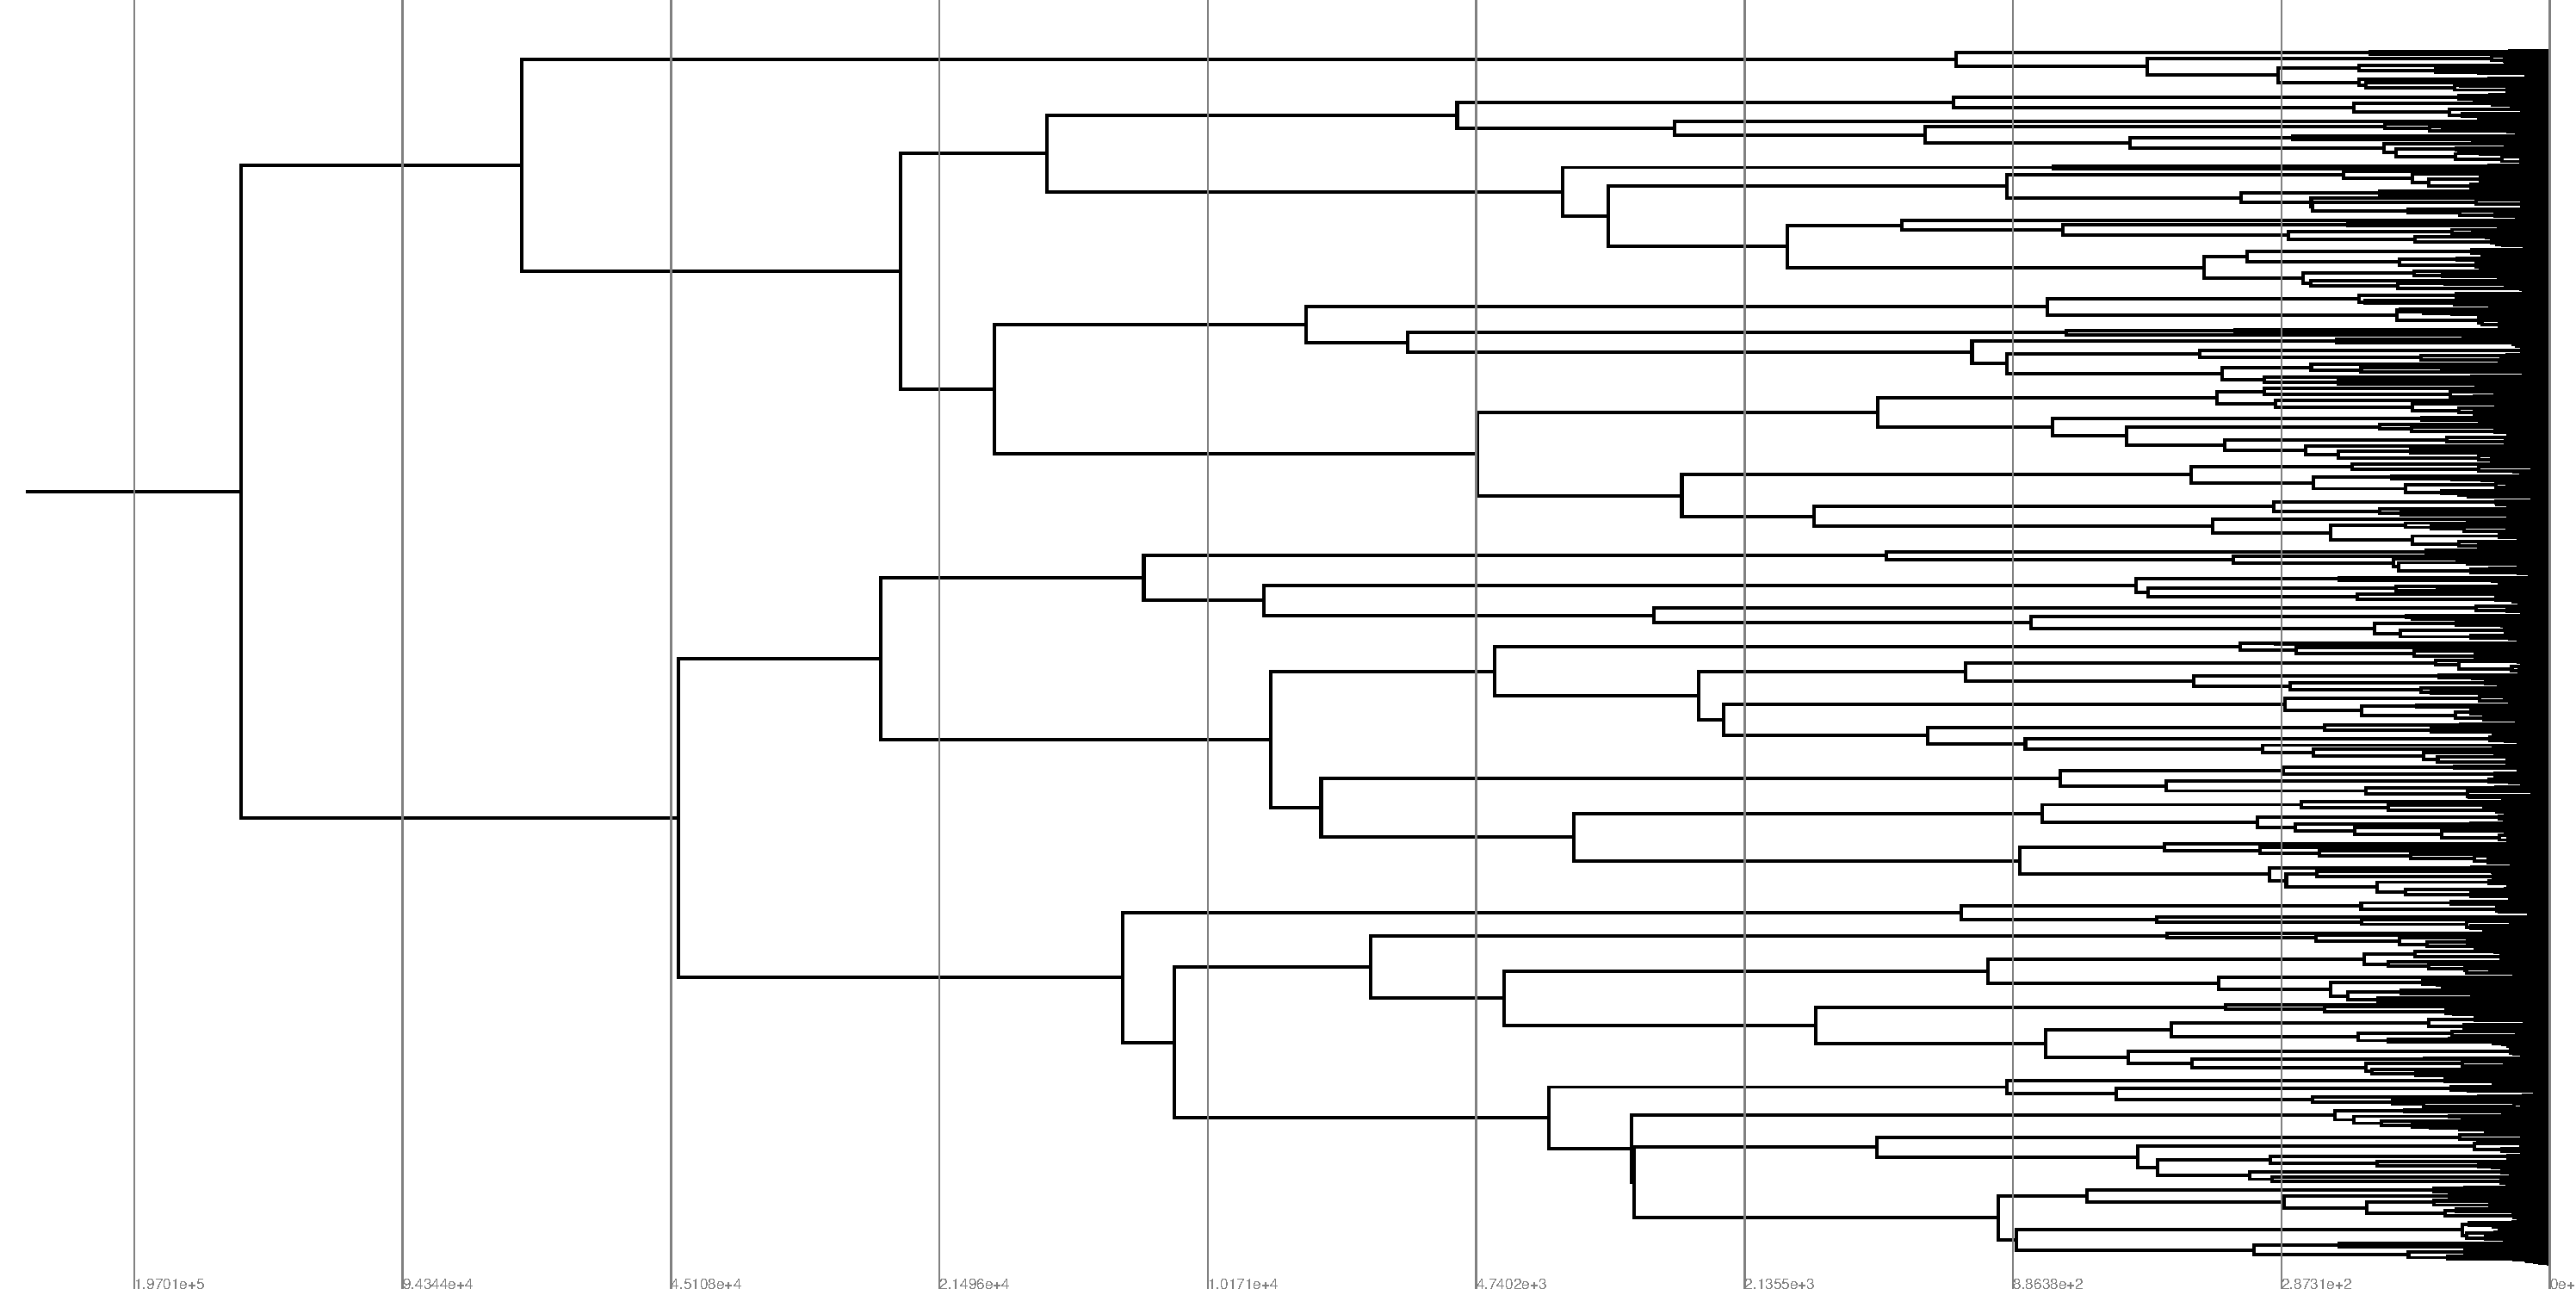
\includegraphics[height=0.12\textheight,width=\textwidth]{img/perfect-tree-phylogenies-log/epoch=7+resolution=3+treatment=0/a=collapsed-phylogeny+epoch=00007+mut_distn=np.random.standard_normal+num_generations=32768+num_islands=1024+num_niches=1+p_island_migration=0.01+p_niche_invasion=3.0517578125e-08+population_size=3276.../8+replicate=0+tournament_size=4+treatment=0+_generation=262144+_index=0+ext=.pdf}
    % \end{noindent}
    \caption{%
      spatial structure}
    % \label{fig:perfect-tree-phylogenies-log:TODO}
  \end{subfigure}
  \hfill
  \begin{subfigure}[b]{1\columnwidth}
    % \begin{noindent}
    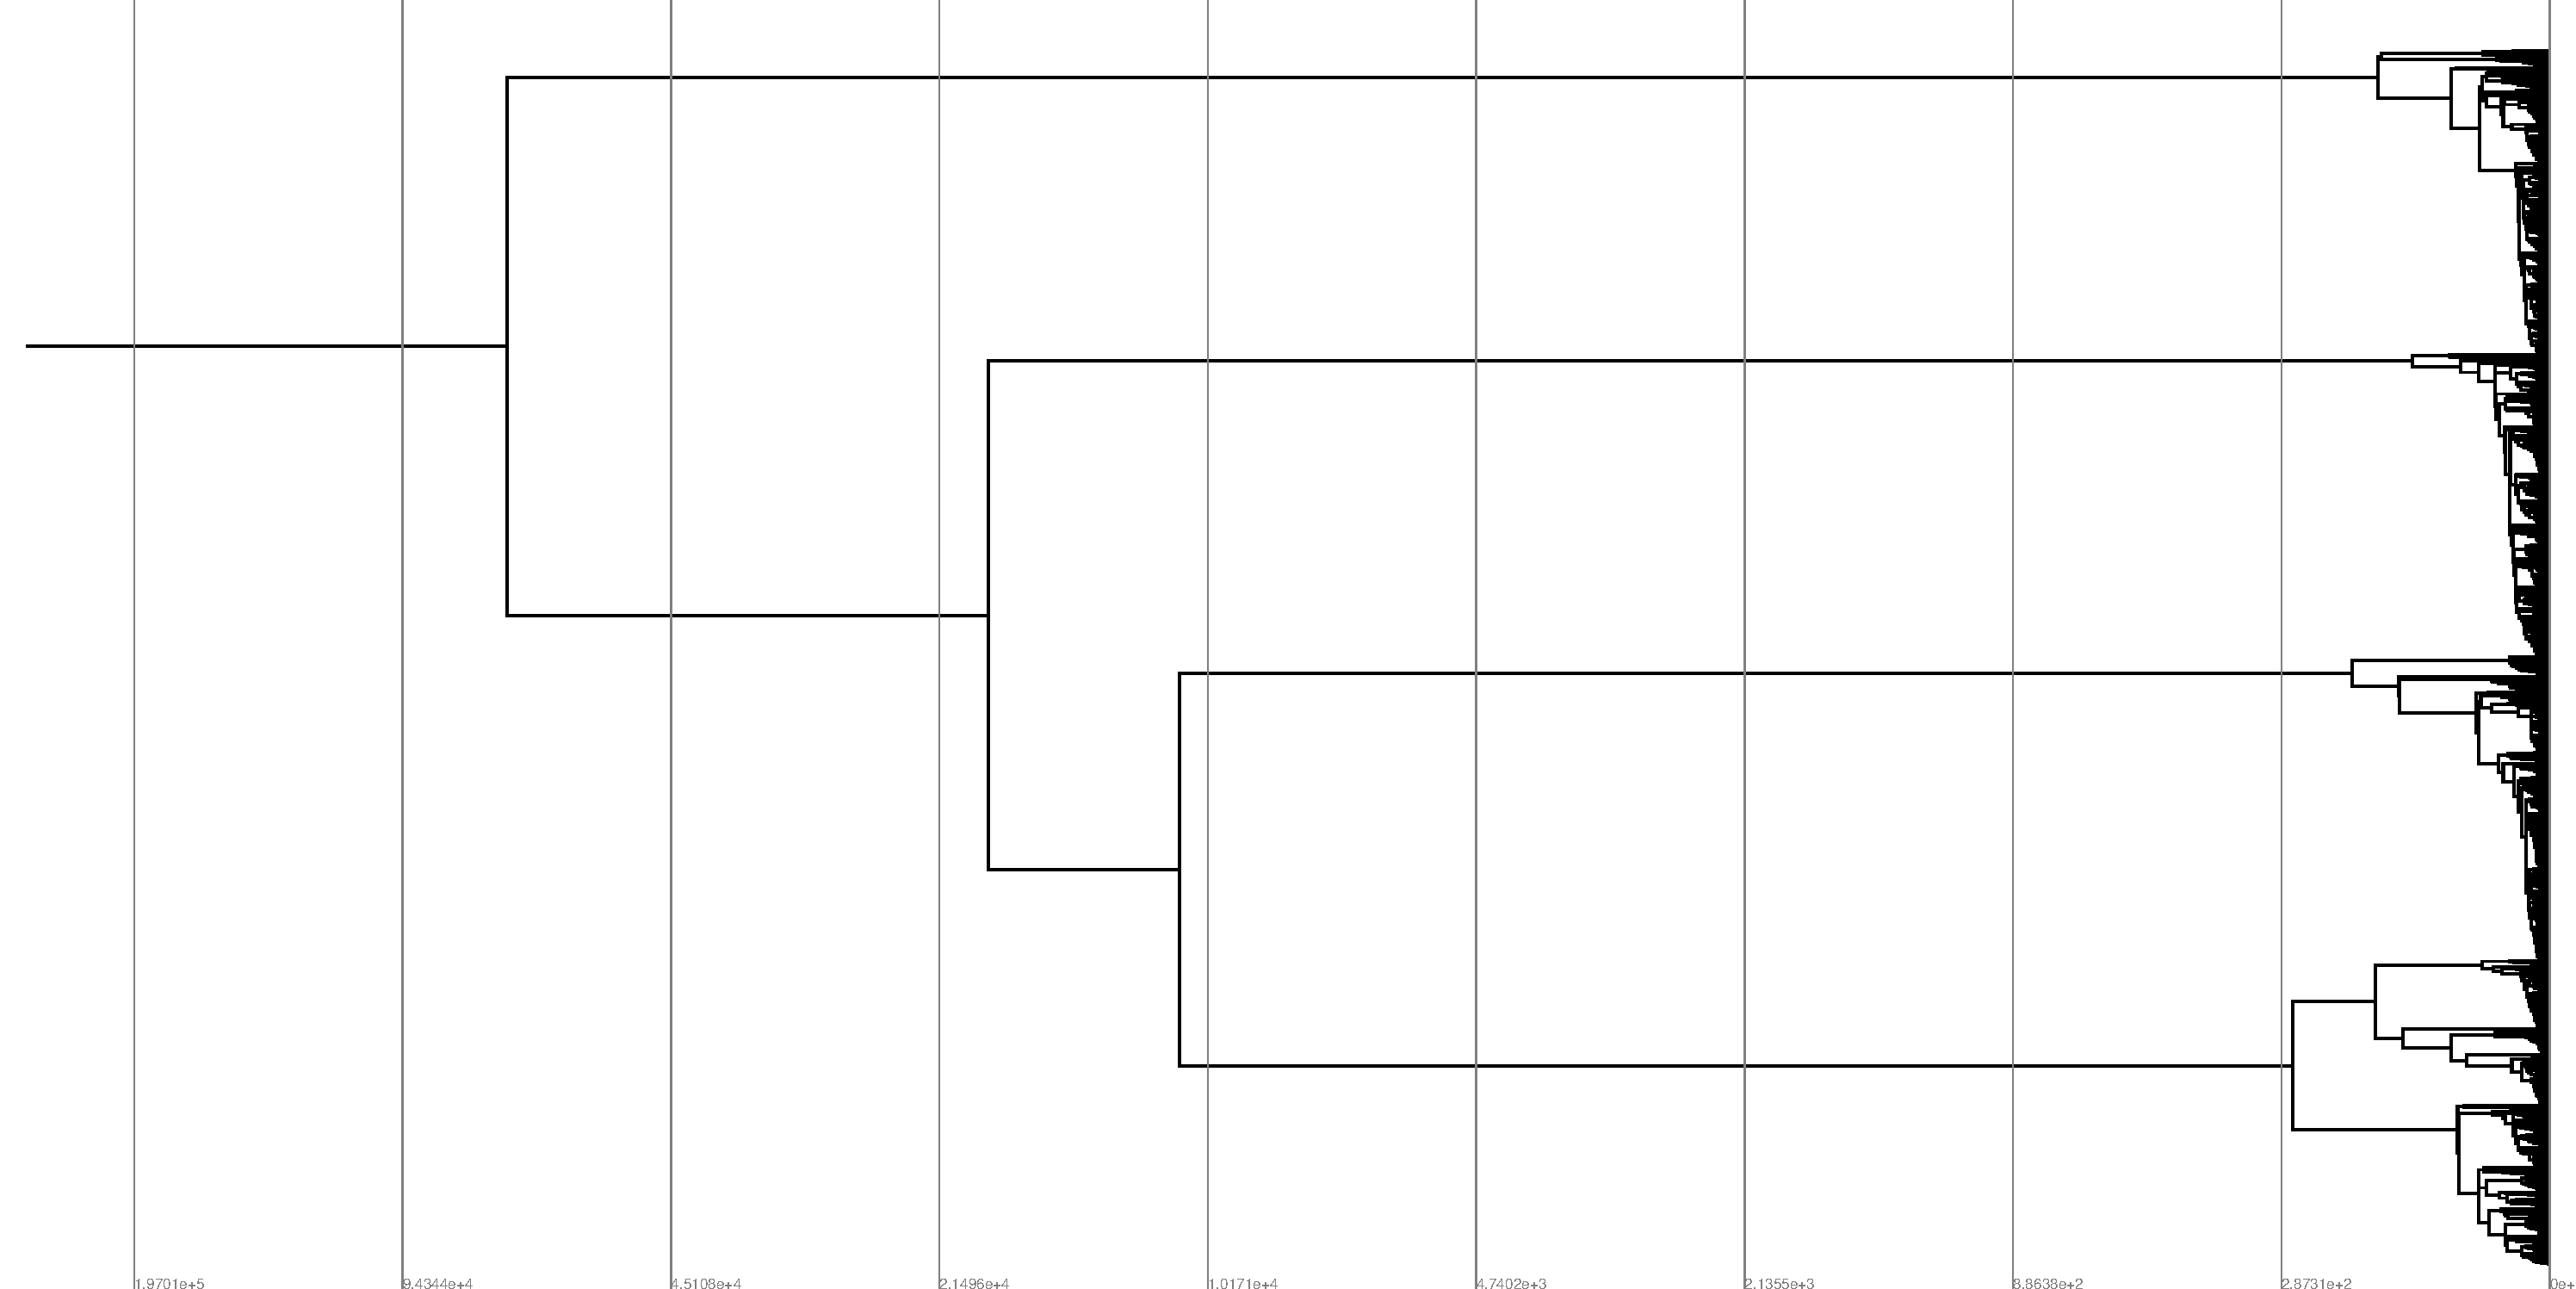
\includegraphics[height=0.12\textheight,width=\textwidth]{img/perfect-tree-phylogenies-log/epoch=7+resolution=3+treatment=10/a=collapsed-phylogeny+epoch=00007+mut_distn=np.random.standard_normal+num_generations=32768+num_islands=1+num_niches=4+p_island_migration=0.01+p_niche_invasion=3.0517578125e-08+population_size=32768+r.../eplicate=0+tournament_size=2+treatment=10+_generation=262144+_index=10+ext=.pdf}
    % \end{noindent}
    \caption{%
      4 niche ecology}
    % \label{fig:perfect-tree-phylogenies-log:TODO}
  \end{subfigure}
  \hfill
  \begin{subfigure}[b]{1\columnwidth}
    % \begin{noindent}
    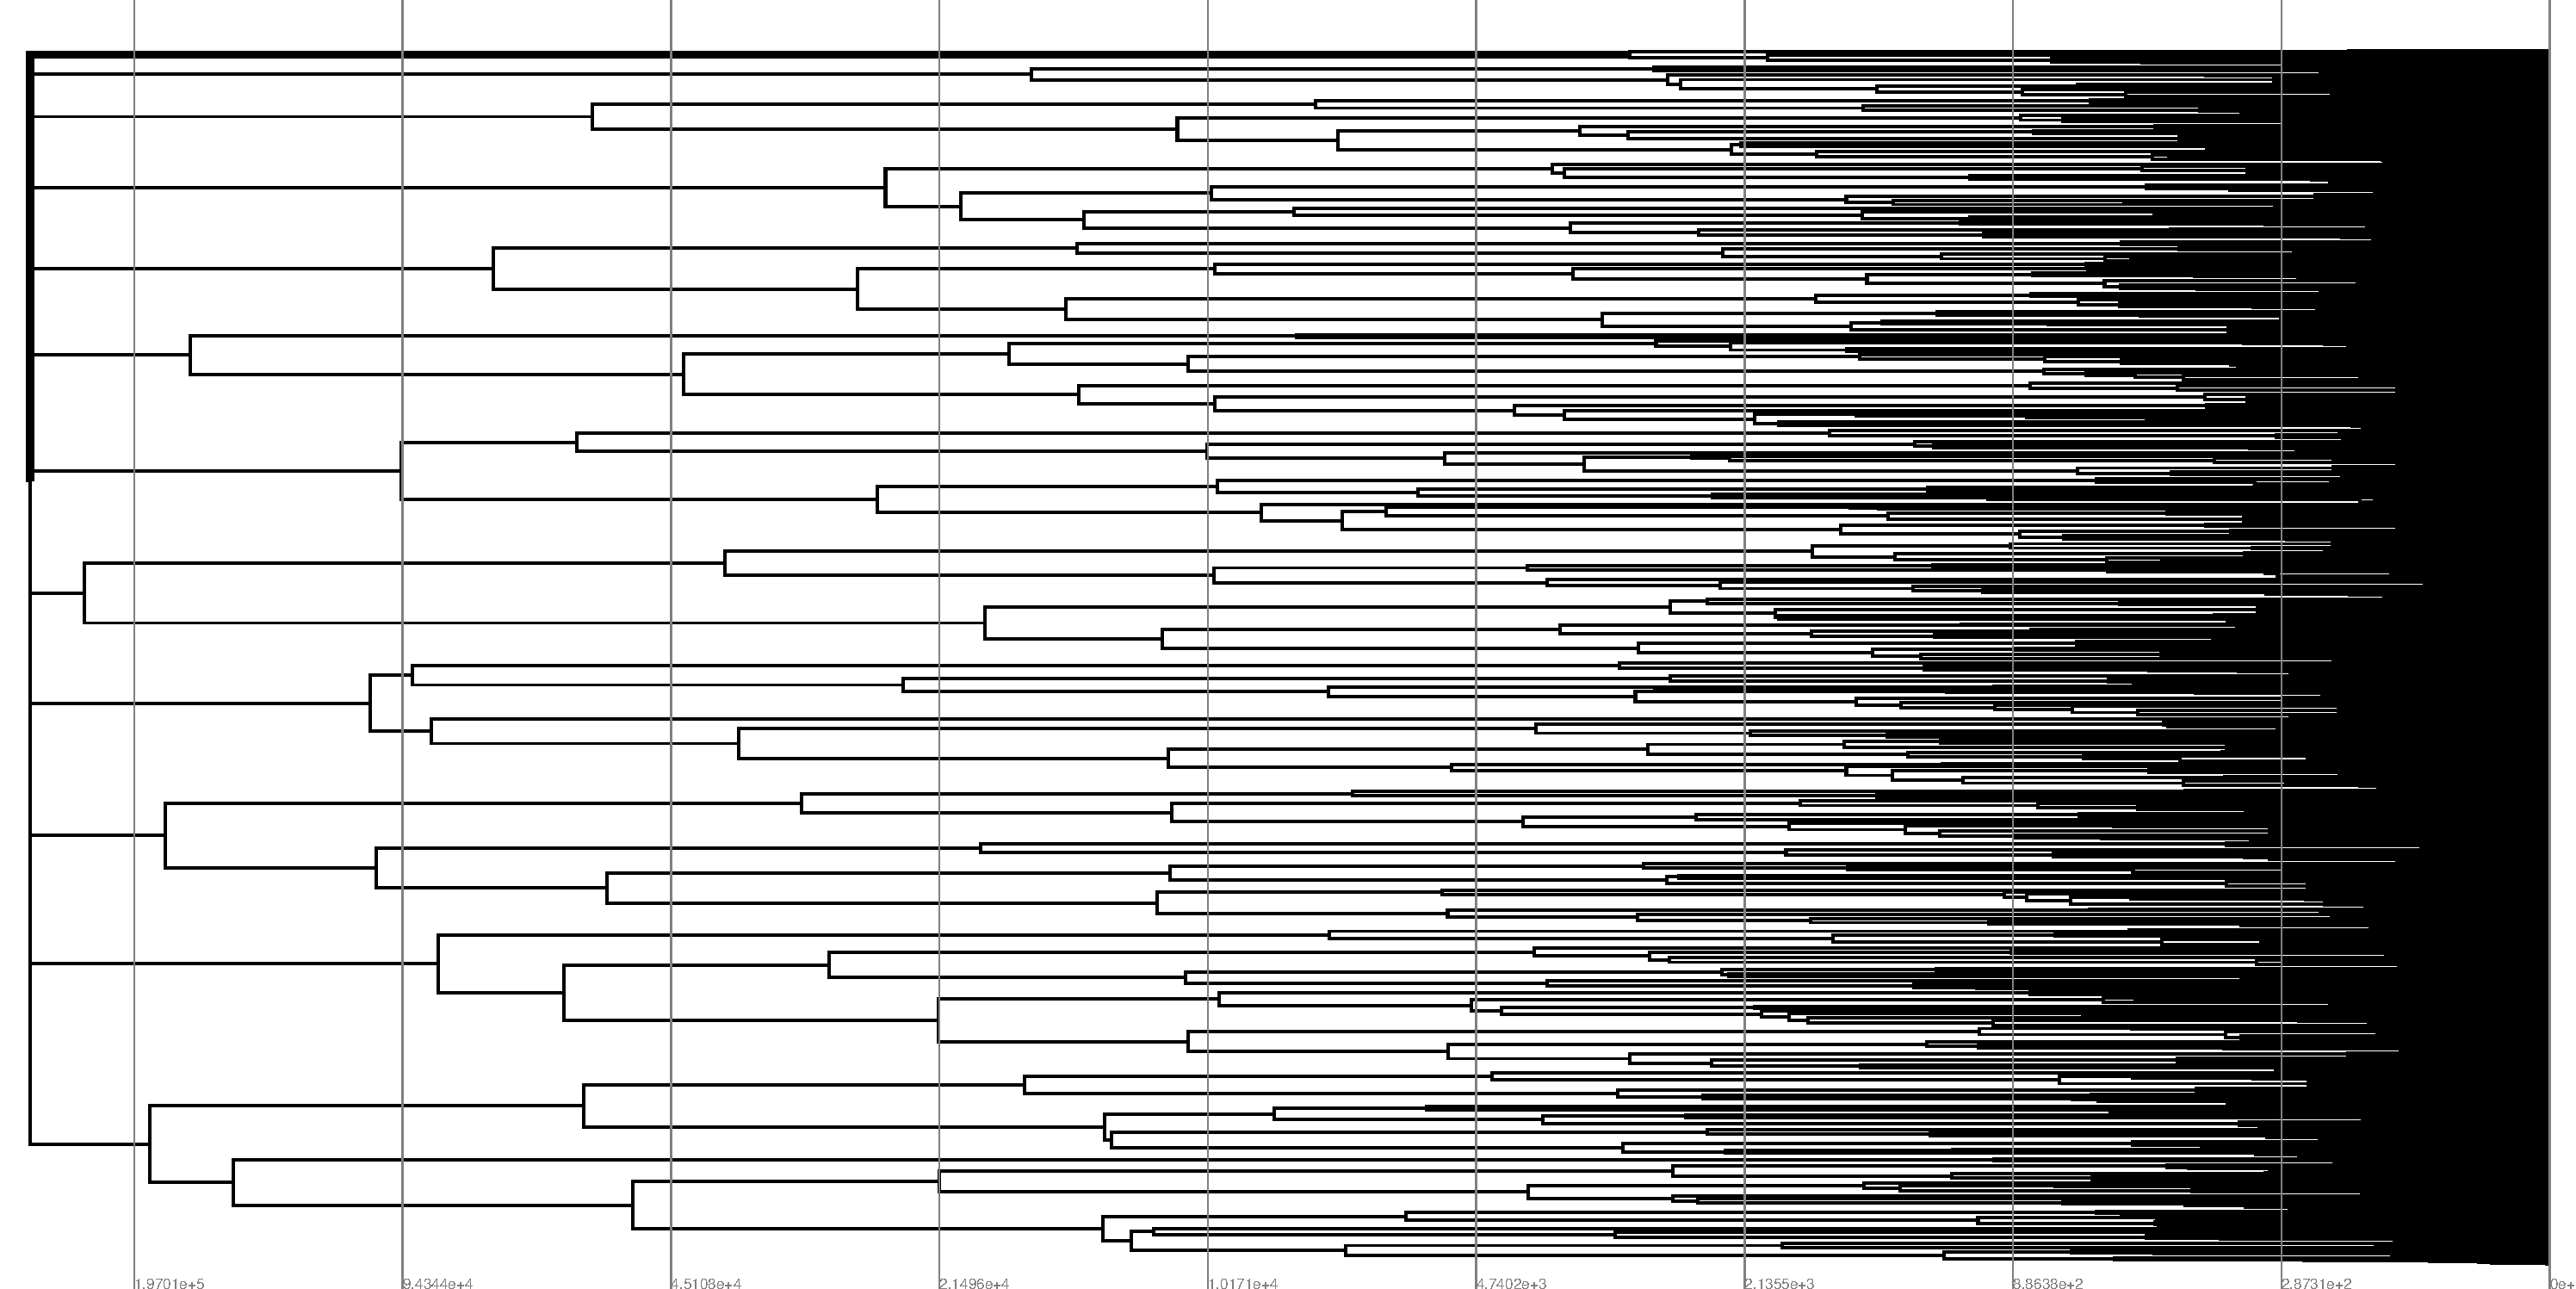
\includegraphics[height=0.12\textheight,width=\textwidth]{img/perfect-tree-phylogenies-log/epoch=7+resolution=3+treatment=12/a=collapsed-phylogeny+epoch=00007+mut_distn=np.random.standard_normal+num_generations=32768+num_islands=1024+num_niches=1+p_island_migration=0.01+p_niche_invasion=3.0517578125e-08+population_size=3276.../8+replicate=0+tournament_size=1+treatment=12+_generation=262144+_index=12+ext=.pdf}
    % \end{noindent}
    \caption{%
      spatial structure weak selection}
    % \label{fig:perfect-tree-phylogenies-log:TODO}
  \end{subfigure}
  \hfill
  \begin{subfigure}[b]{1\columnwidth}
    % \begin{noindent}
    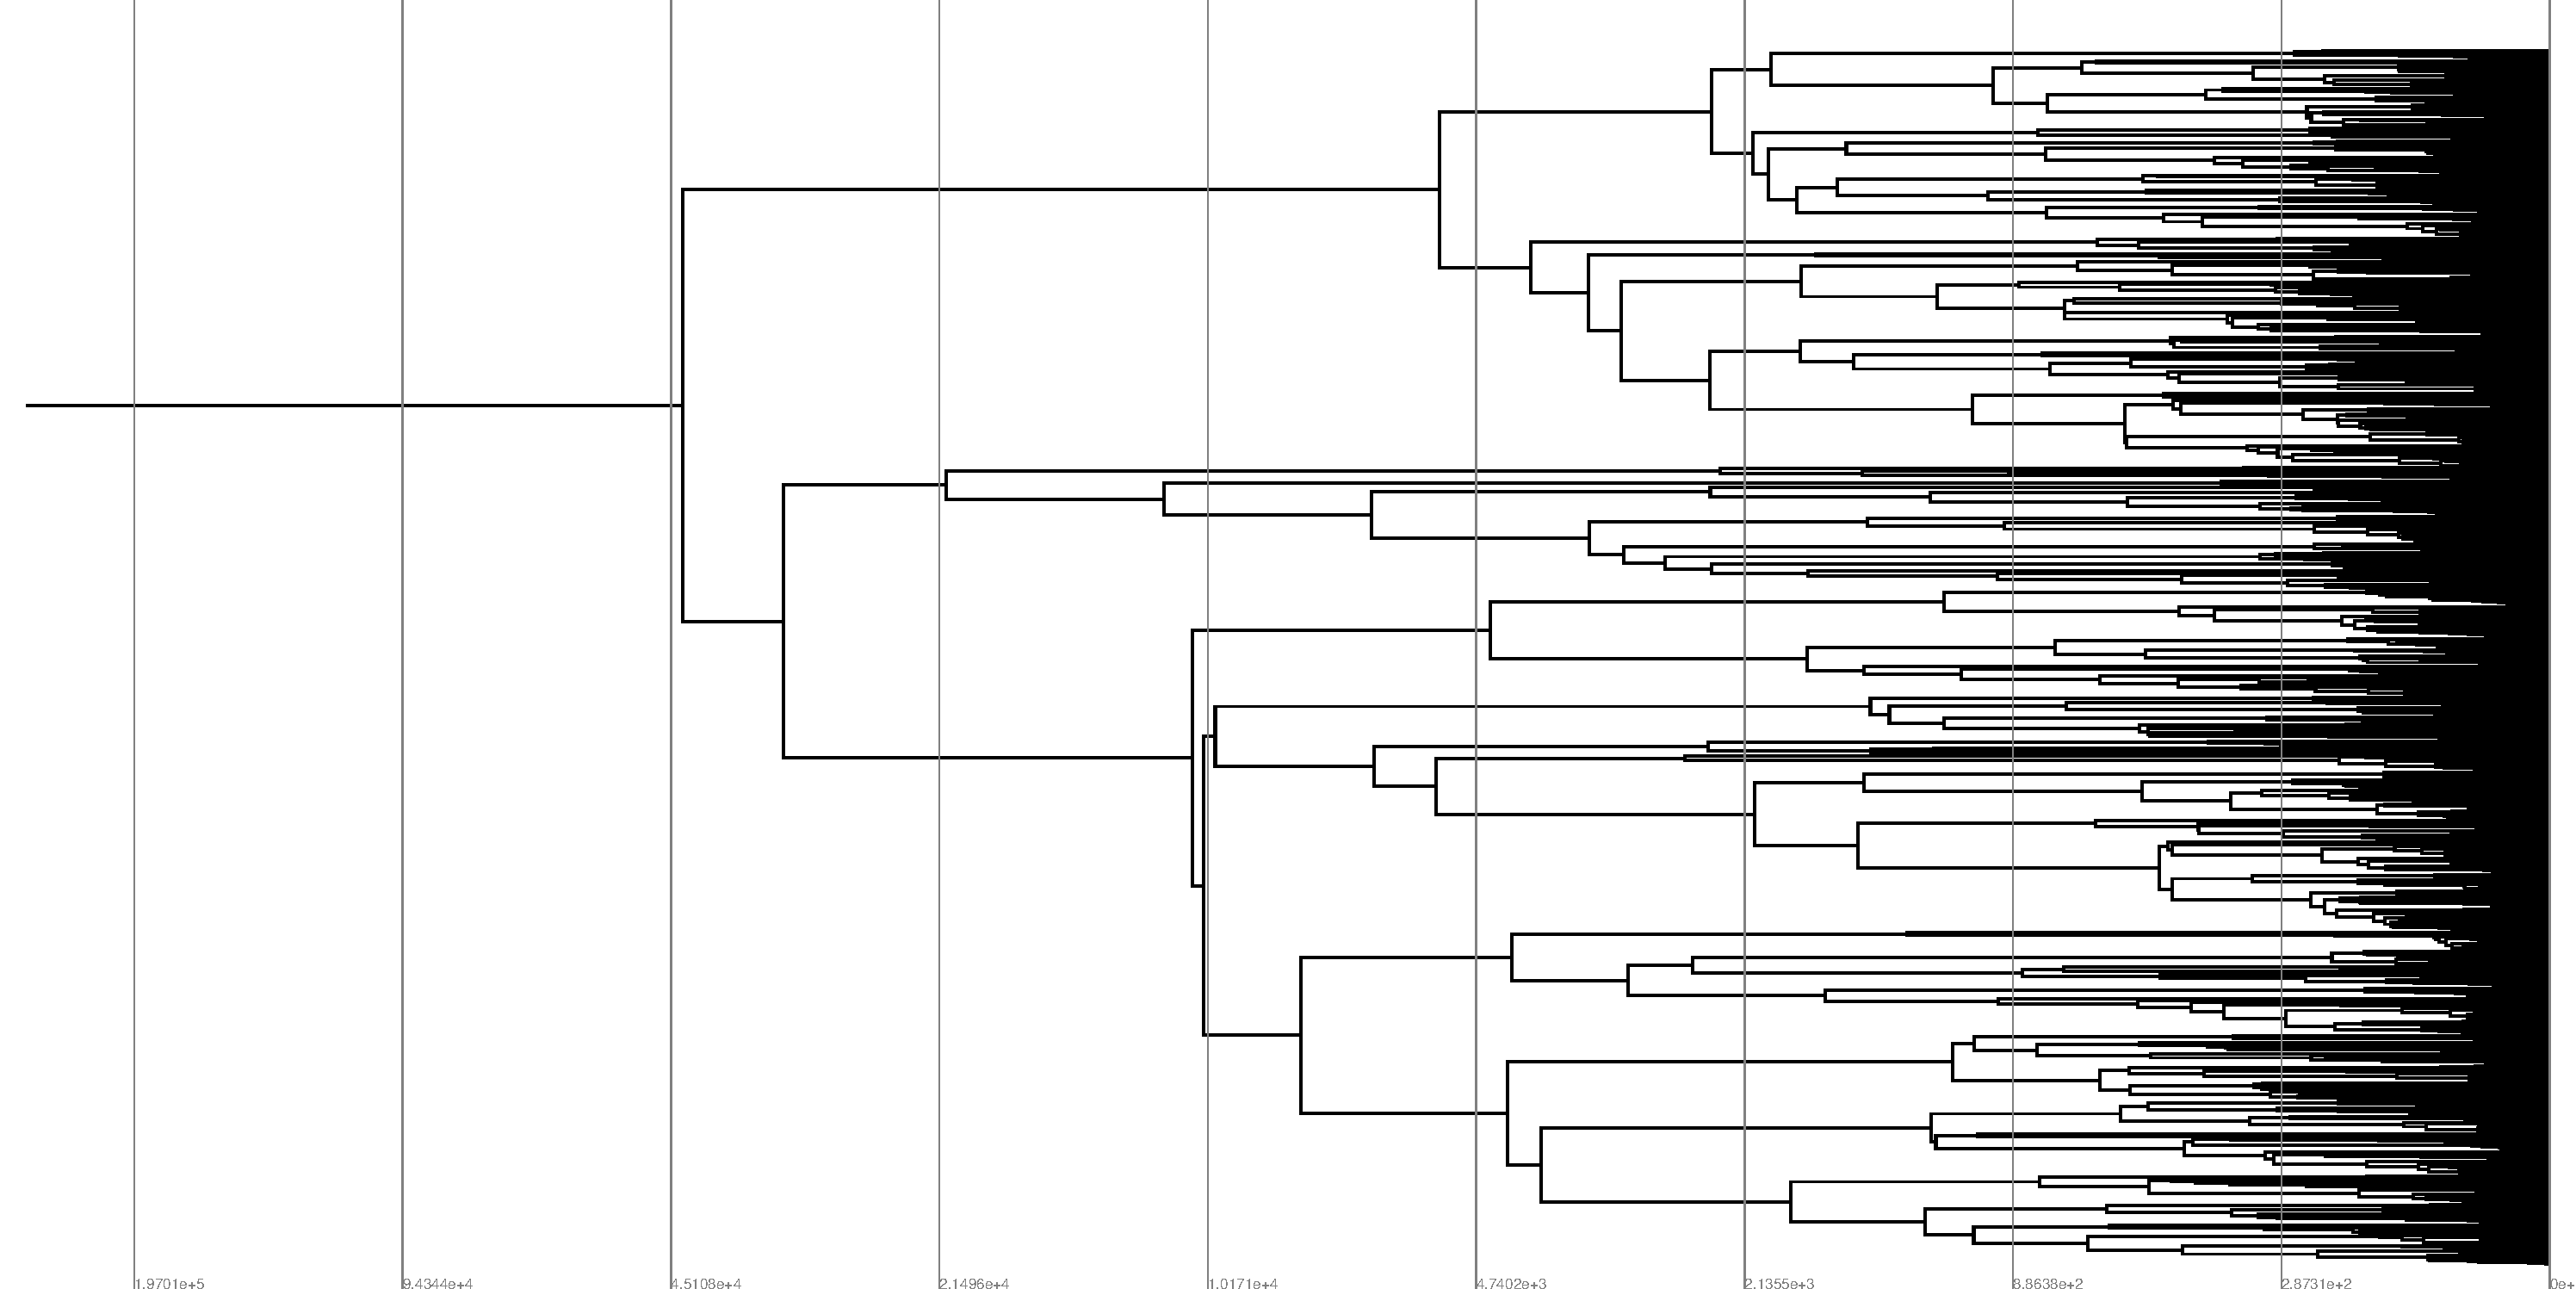
\includegraphics[height=0.12\textheight,width=\textwidth]{img/perfect-tree-phylogenies-log/epoch=7+resolution=3+treatment=14/a=collapsed-phylogeny+epoch=00007+mut_distn=np.random.standard_normal+num_generations=32768+num_islands=1+num_niches=1+p_island_migration=0.01+p_niche_invasion=3.0517578125e-08+population_size=32768+r.../eplicate=0+tournament_size=1+treatment=14+_generation=262144+_index=14+ext=.pdf}
    % \end{noindent}
    \caption{%
      weak selection}
    % \label{fig:perfect-tree-phylogenies-log:TODO}
  \end{subfigure}
  \hfill
  \begin{subfigure}[b]{1\columnwidth}
    % \begin{noindent}
    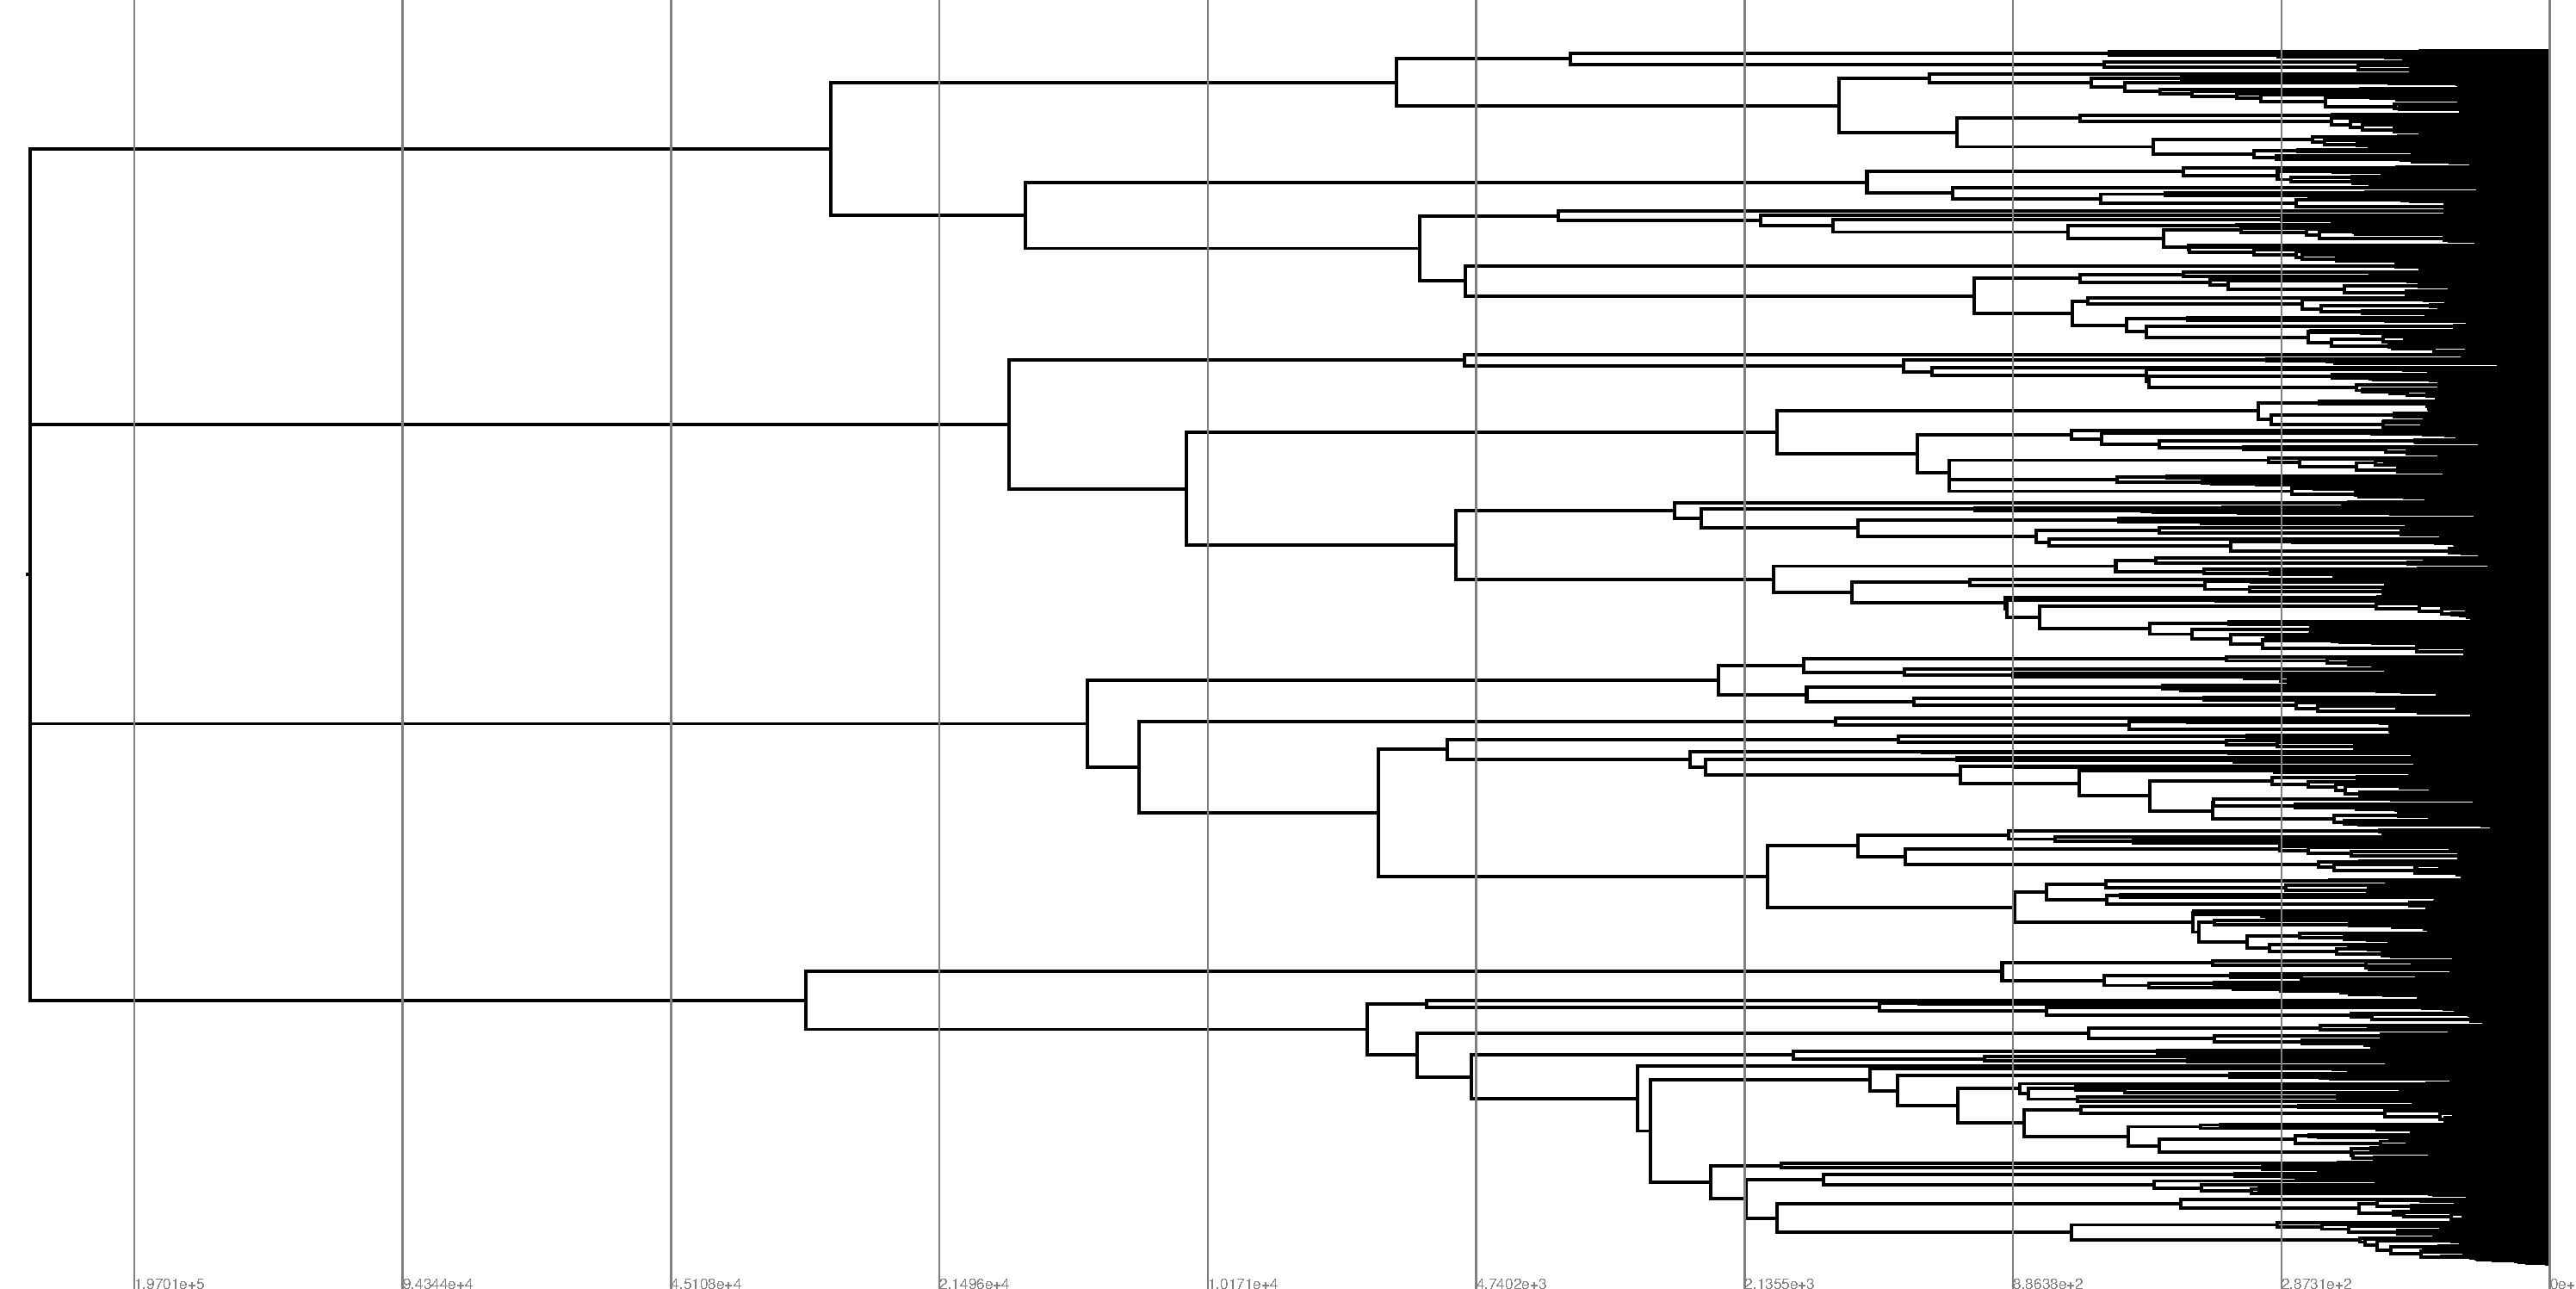
\includegraphics[height=0.12\textheight,width=\textwidth]{img/perfect-tree-phylogenies-log/epoch=7+resolution=3+treatment=16/a=collapsed-phylogeny+epoch=00007+mut_distn=np.random.standard_normal+num_generations=32768+num_islands=1+num_niches=4+p_island_migration=0.01+p_niche_invasion=3.0517578125e-08+population_size=32768+r.../eplicate=0+tournament_size=1+treatment=16+_generation=262144+_index=16+ext=.pdf}
    % \end{noindent}
    \caption{%
      weak selection 4 niche ecology}
    % \label{fig:perfect-tree-phylogenies-log:TODO}
  \end{subfigure}
  \hfill
  \begin{subfigure}[b]{1\columnwidth}
    % \begin{noindent}
    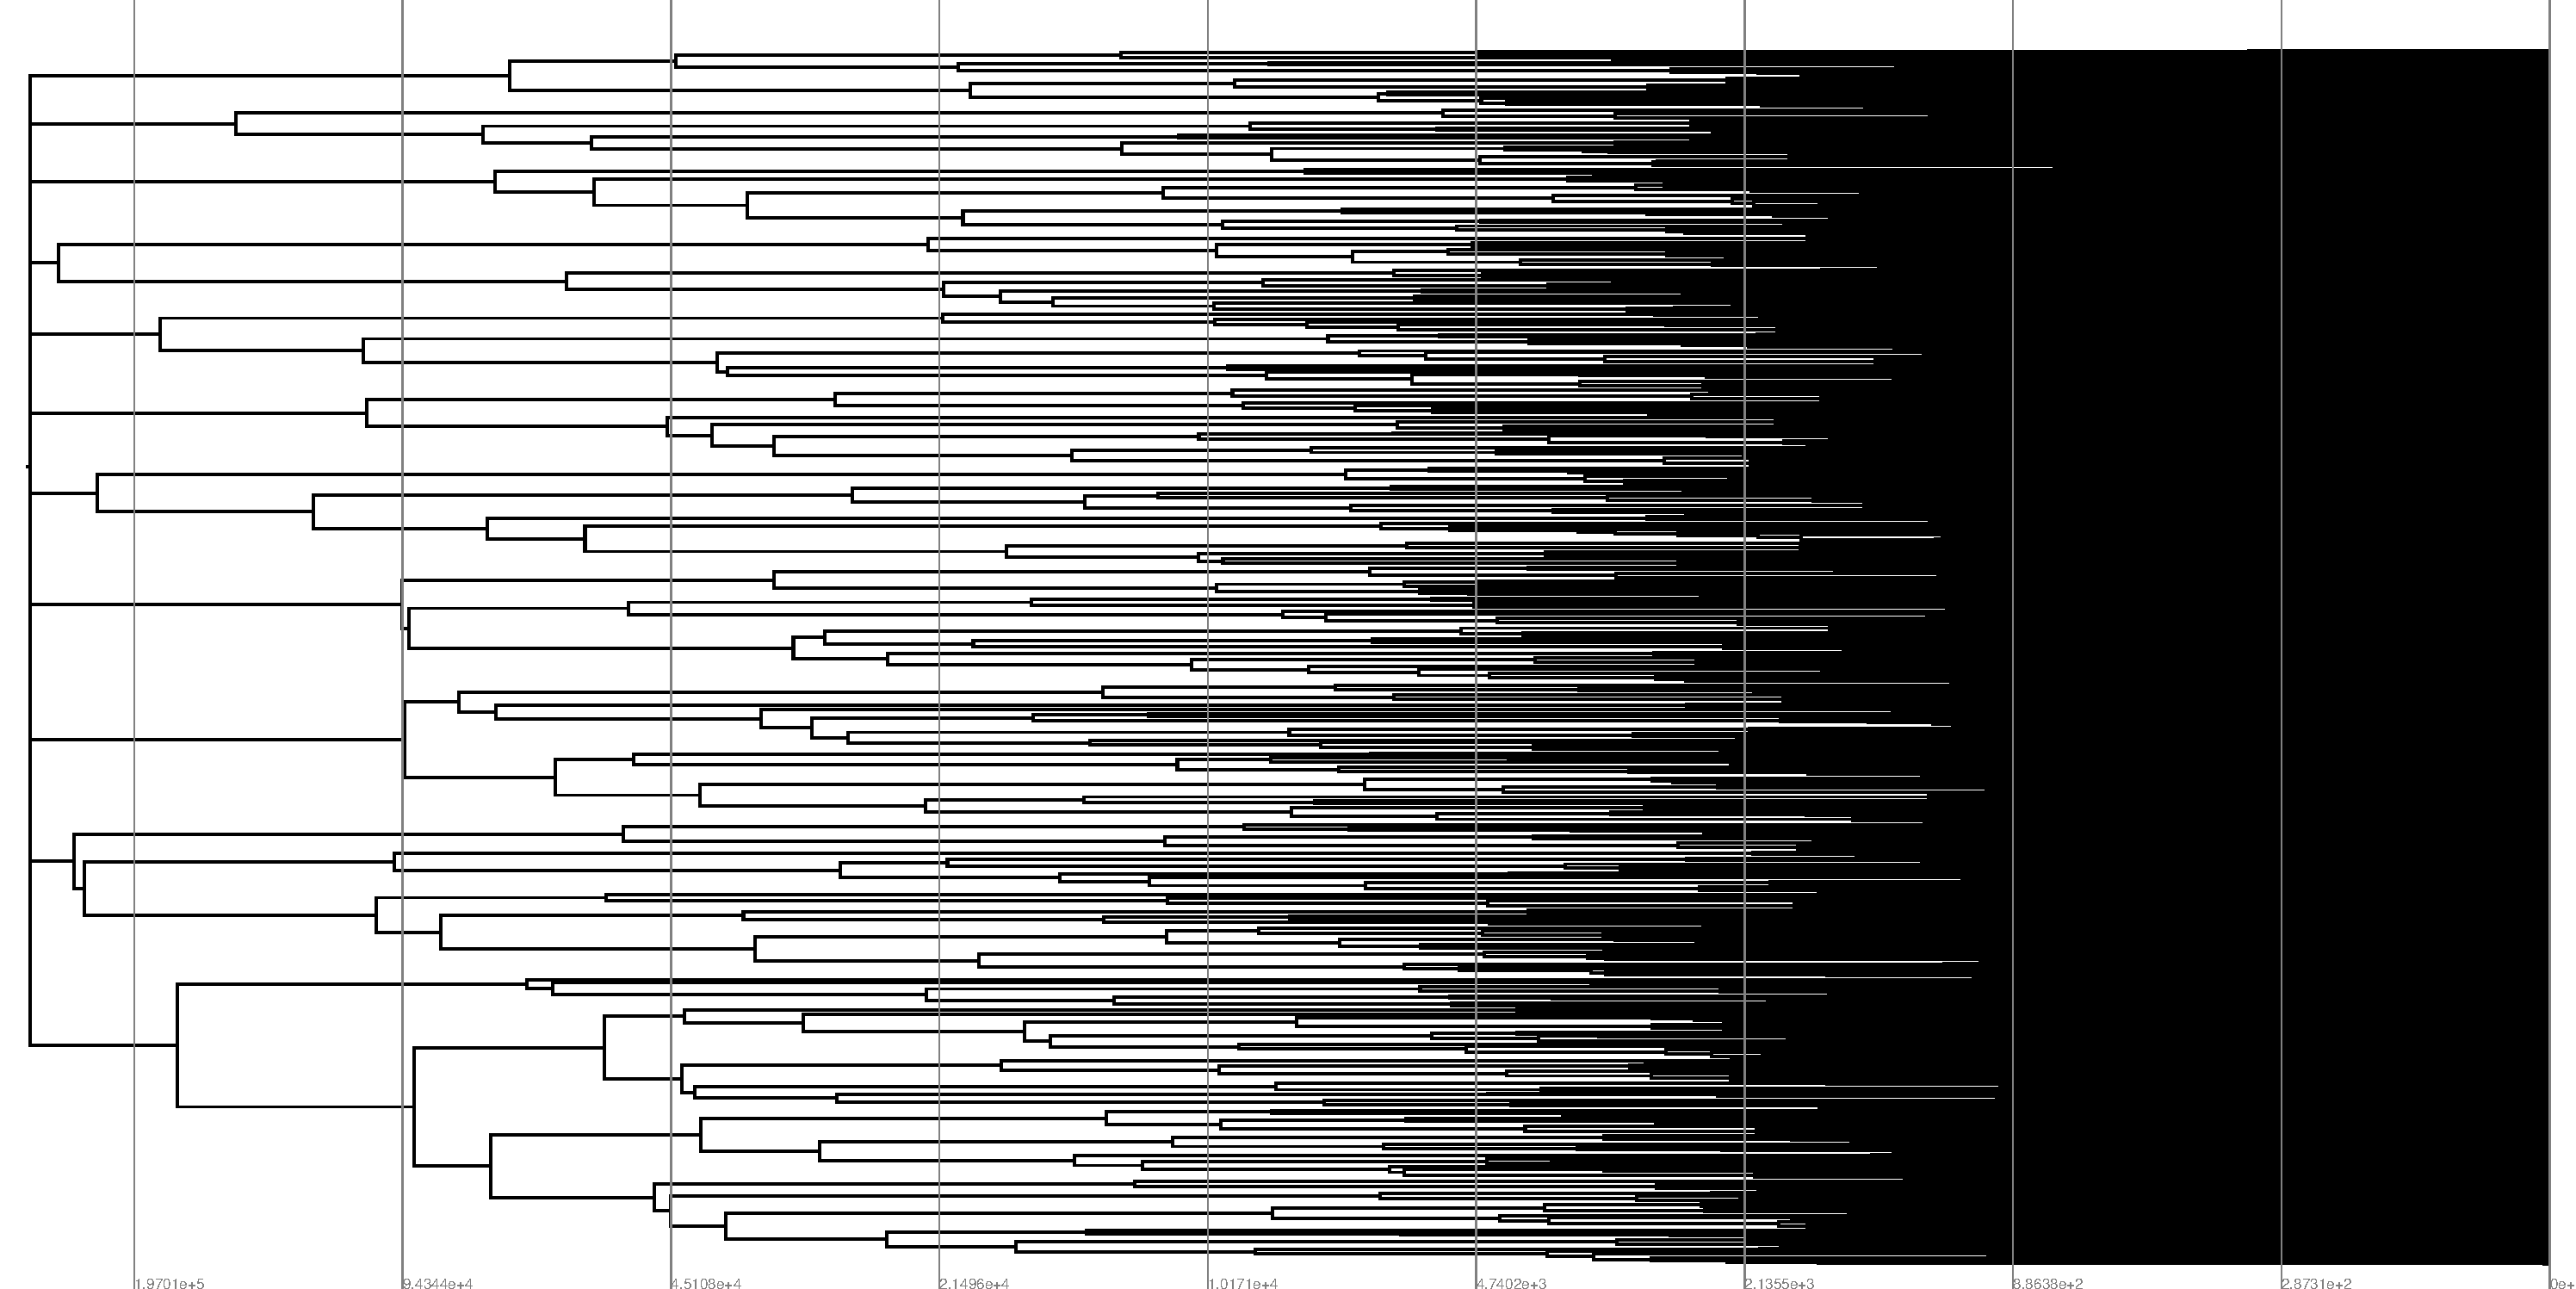
\includegraphics[height=0.12\textheight,width=\textwidth]{img/perfect-tree-phylogenies-log/epoch=7+resolution=3+treatment=18/a=collapsed-phylogeny+epoch=00007+mut_distn=np.random.standard_normal+num_generations=32768+num_islands=1024+num_niches=8+p_island_migration=0.01+p_niche_invasion=3.0517578125e-08+population_size=3276.../8+replicate=0+tournament_size=2+treatment=18+_generation=262144+_index=18+ext=.pdf}
    % \end{noindent}
    \caption{%
      spatial structure 8 niche ecology}
    % \label{fig:perfect-tree-phylogenies-log:TODO}
  \end{subfigure}

  \begin{subfigure}[b]{1\columnwidth}
    % \begin{noindent}
    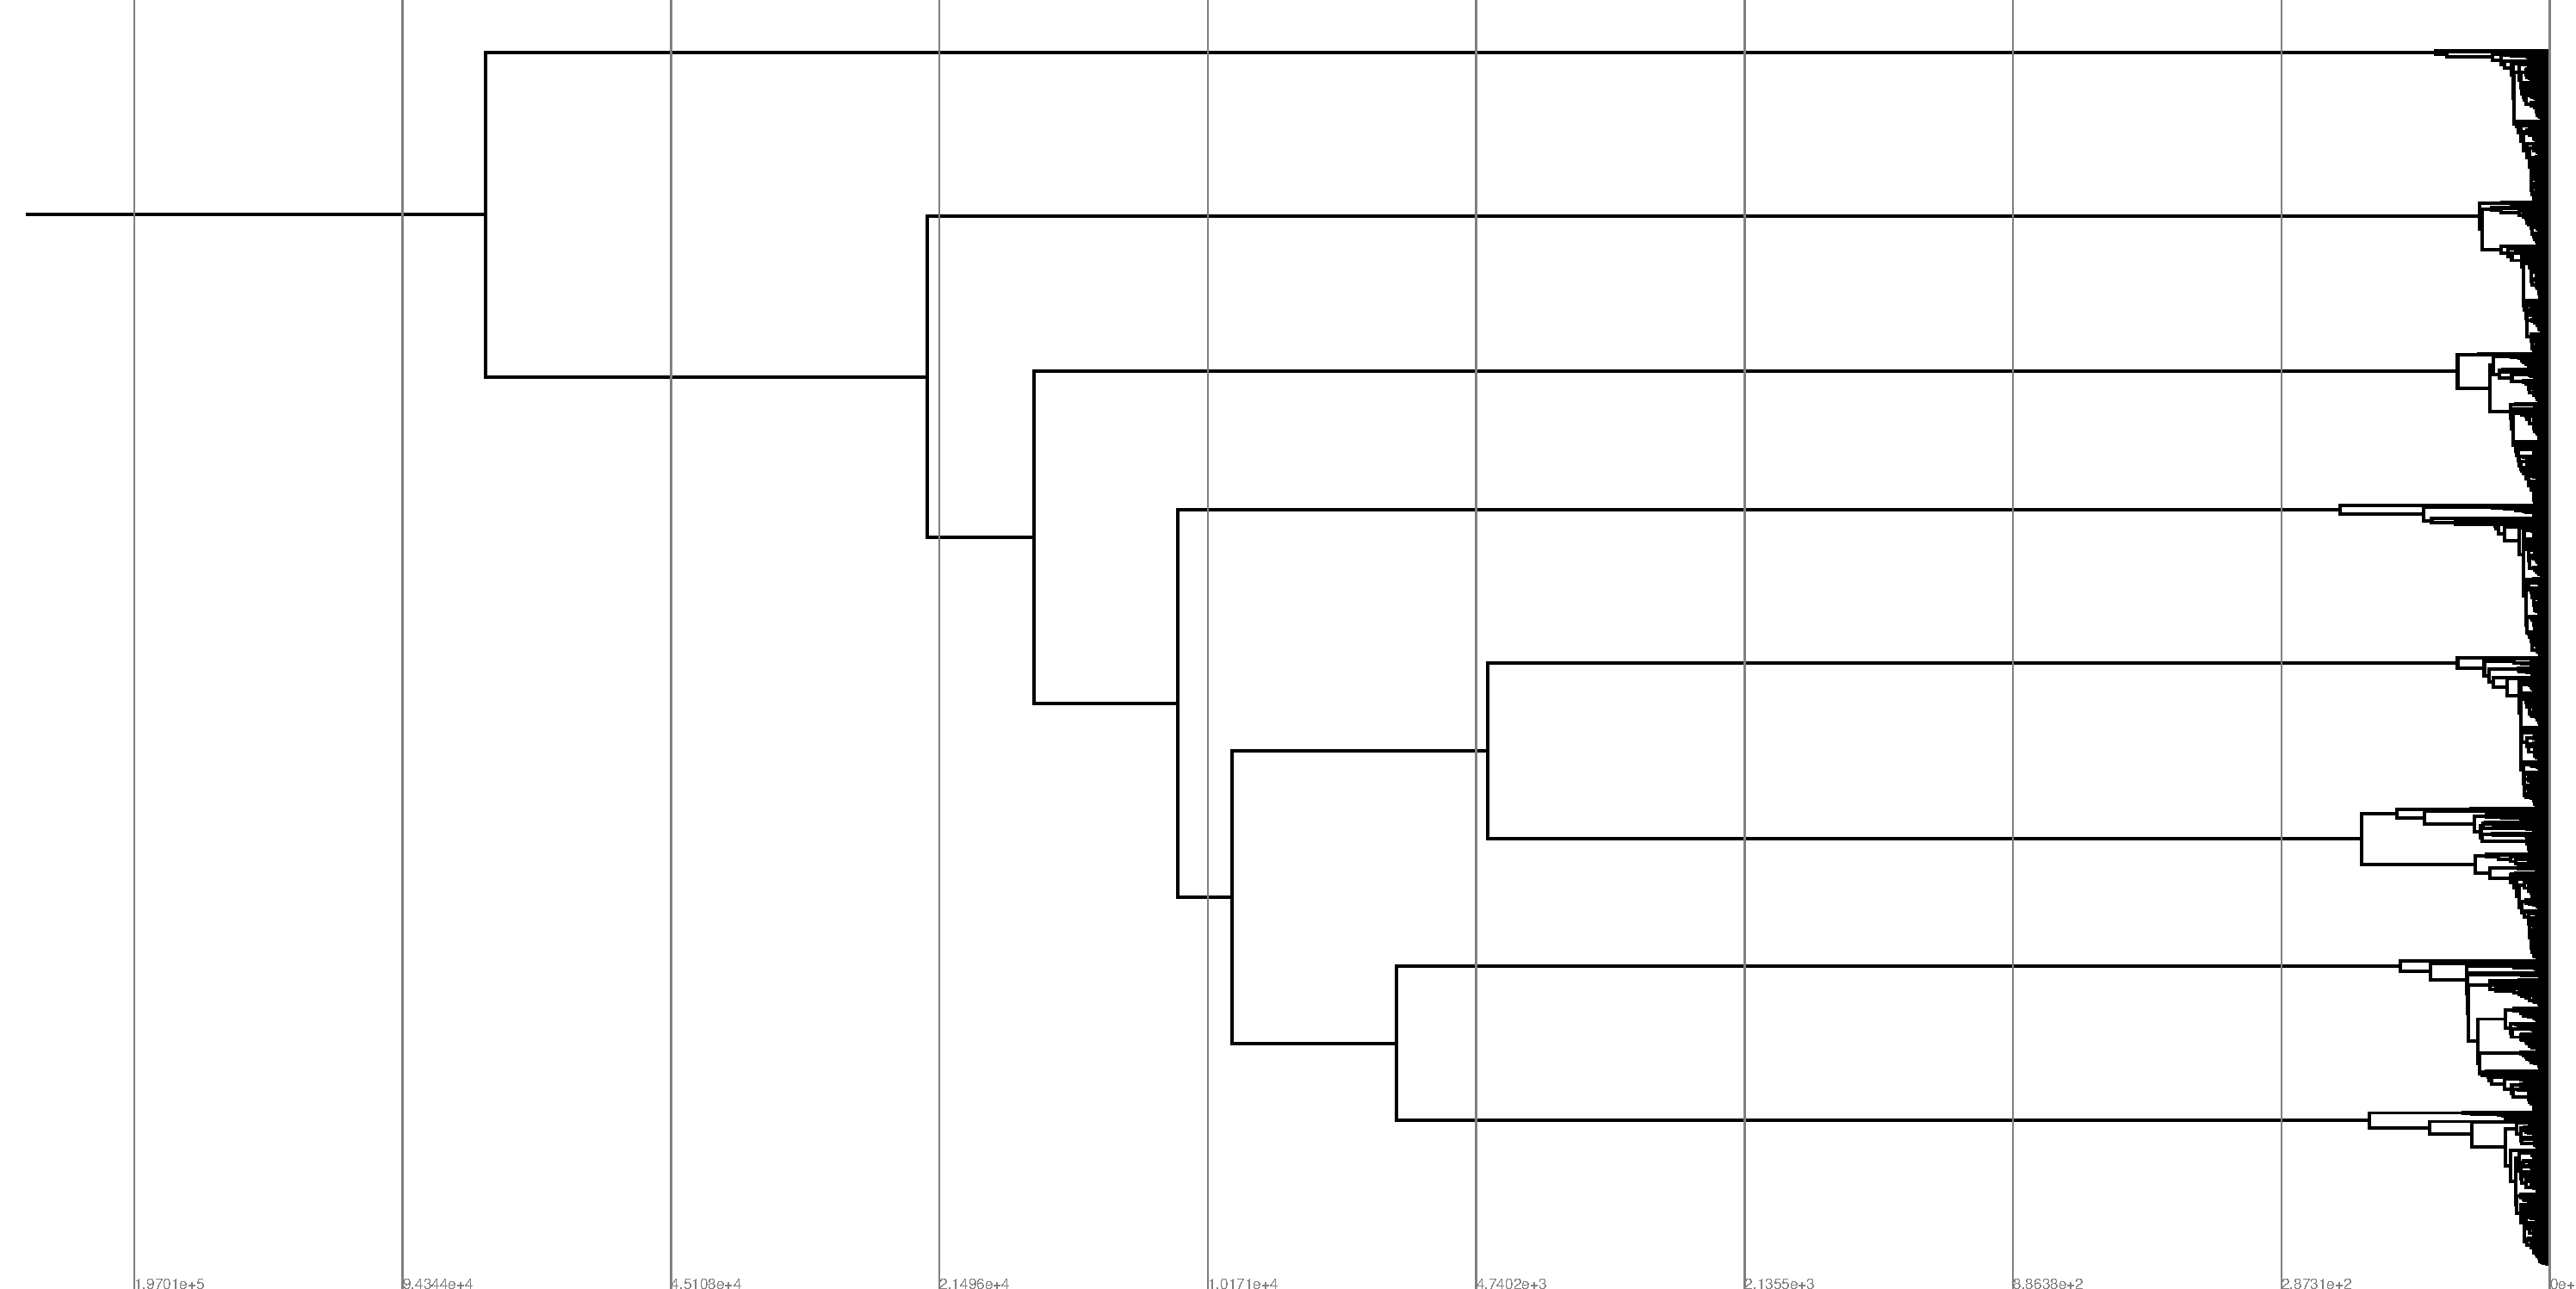
\includegraphics[height=0.12\textheight,width=\textwidth]{img/perfect-tree-phylogenies-log/epoch=7+resolution=3+treatment=20/a=collapsed-phylogeny+epoch=00007+mut_distn=np.random.standard_normal+num_generations=32768+num_islands=1+num_niches=8+p_island_migration=0.01+p_niche_invasion=3.0517578125e-08+population_size=32768+r.../eplicate=0+tournament_size=2+treatment=20+_generation=262144+_index=20+ext=.pdf}
    % \end{noindent}
    \caption{%
      8 niche ecology}
    % \label{fig:perfect-tree-phylogenies-log:TODO}
  \end{subfigure}
  \hfill
  \begin{subfigure}[b]{1\columnwidth}
    % \begin{noindent}
    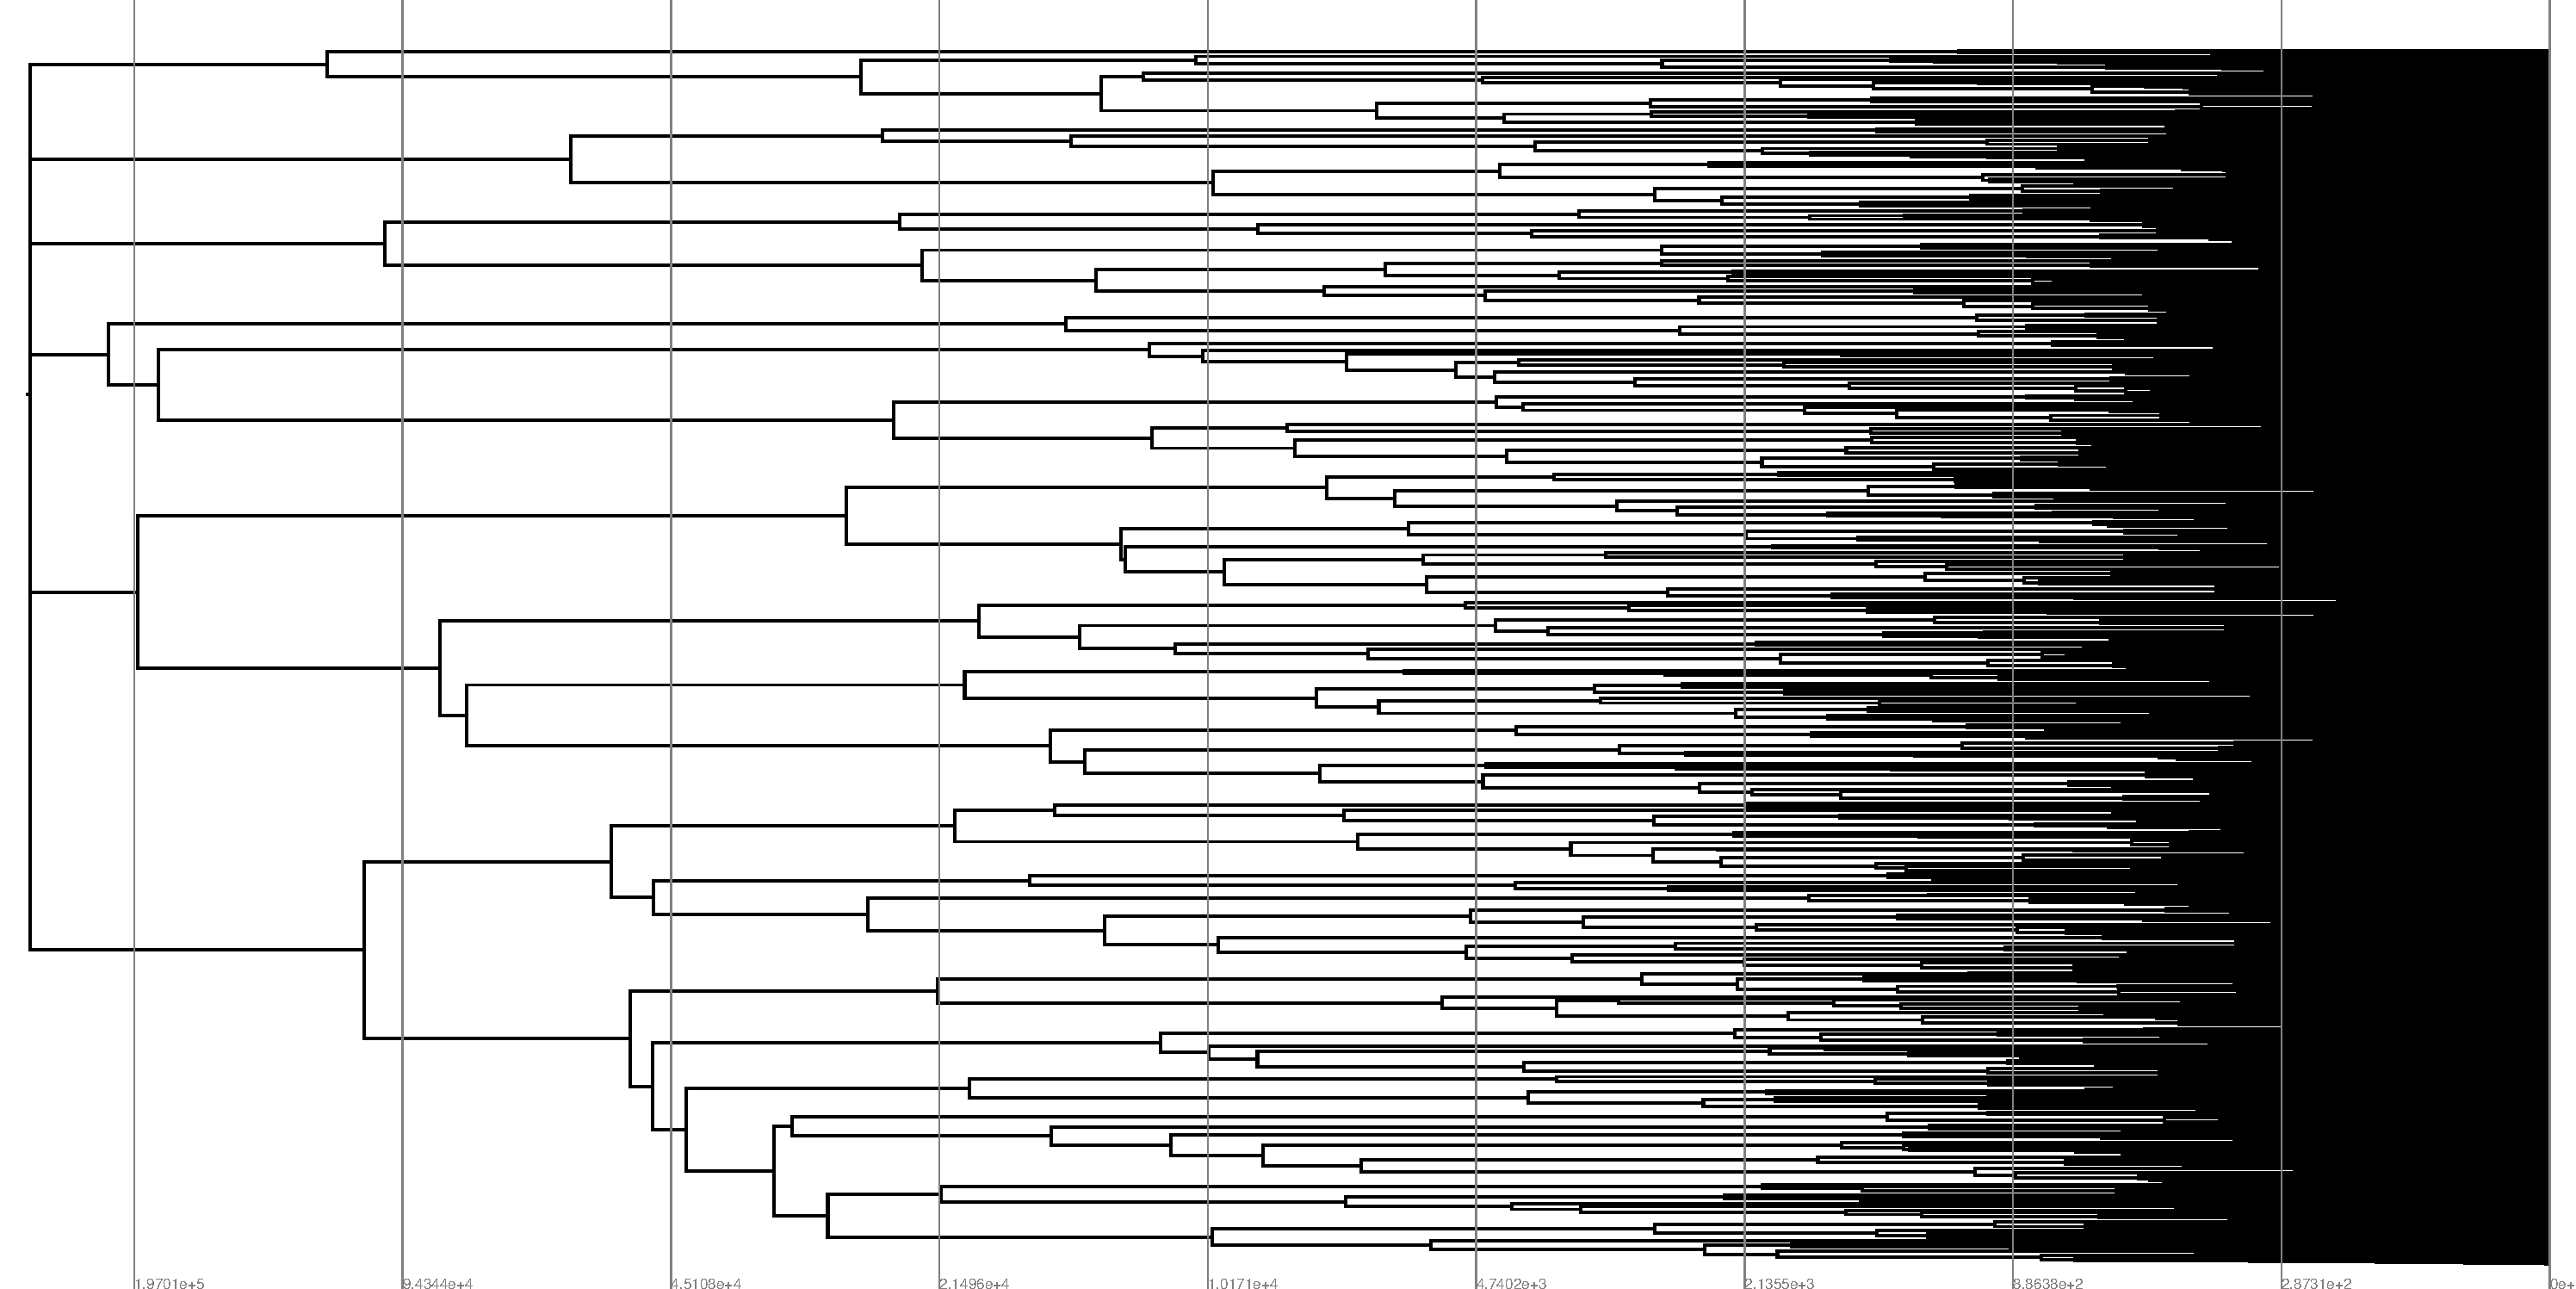
\includegraphics[height=0.12\textheight,width=\textwidth]{img/perfect-tree-phylogenies-log/epoch=7+resolution=3+treatment=22/a=collapsed-phylogeny+epoch=00007+mut_distn=np.random.standard_normal+num_generations=32768+num_islands=1024+num_niches=4+p_island_migration=0.01+p_niche_invasion=3.0517578125e-08+population_size=3276.../8+replicate=0+tournament_size=2+treatment=22+_generation=262144+_index=22+ext=.pdf}
    % \end{noindent}
    \caption{%
      spatial structure 4 niche ecology}
    % \label{fig:perfect-tree-phylogenies-log:TODO}
  \end{subfigure}
  \hfill
  \begin{subfigure}[b]{1\columnwidth}
    % \begin{noindent}
    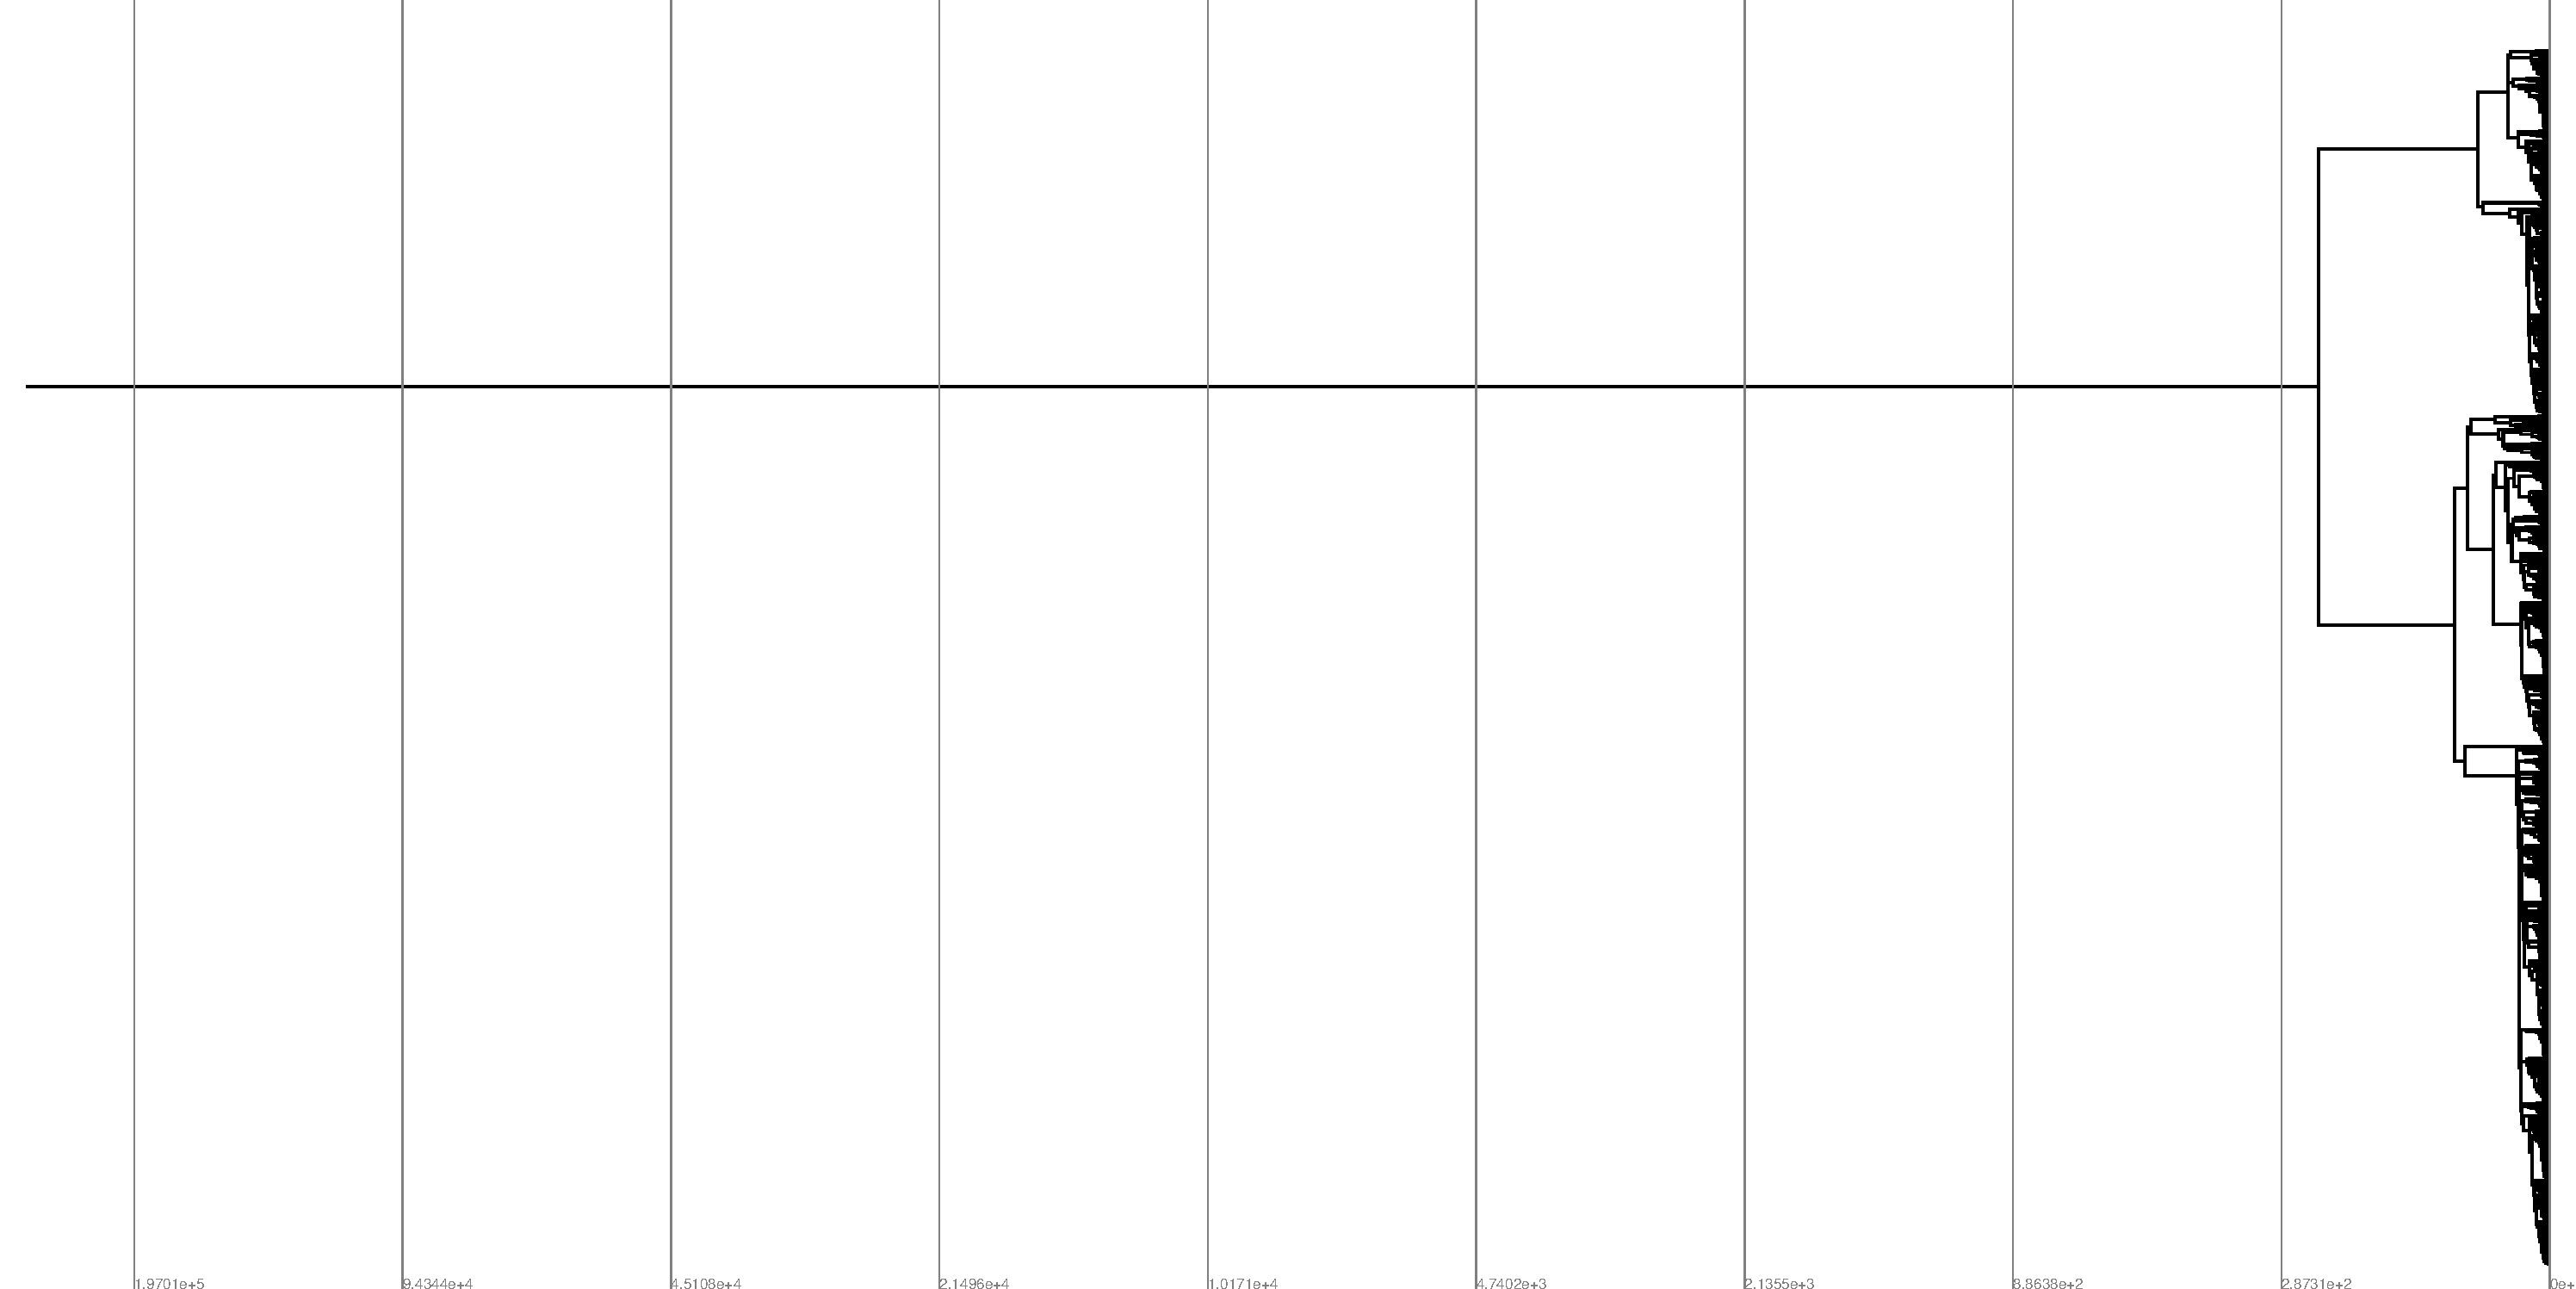
\includegraphics[height=0.12\textheight,width=\textwidth]{img/perfect-tree-phylogenies-log/epoch=7+resolution=3+treatment=2/a=collapsed-phylogeny+epoch=00007+mut_distn=np.random.standard_normal+num_generations=32768+num_islands=1+num_niches=1+p_island_migration=0.01+p_niche_invasion=3.0517578125e-08+population_size=32768+r.../eplicate=0+tournament_size=4+treatment=2+_generation=262144+_index=2+ext=.pdf}
    % \end{noindent}
    \caption{%
      strong selection}
    % \label{fig:perfect-tree-phylogenies-log:TODO}
  \end{subfigure}
  \hfill
  \begin{subfigure}[b]{1\columnwidth}
    % \begin{noindent}
    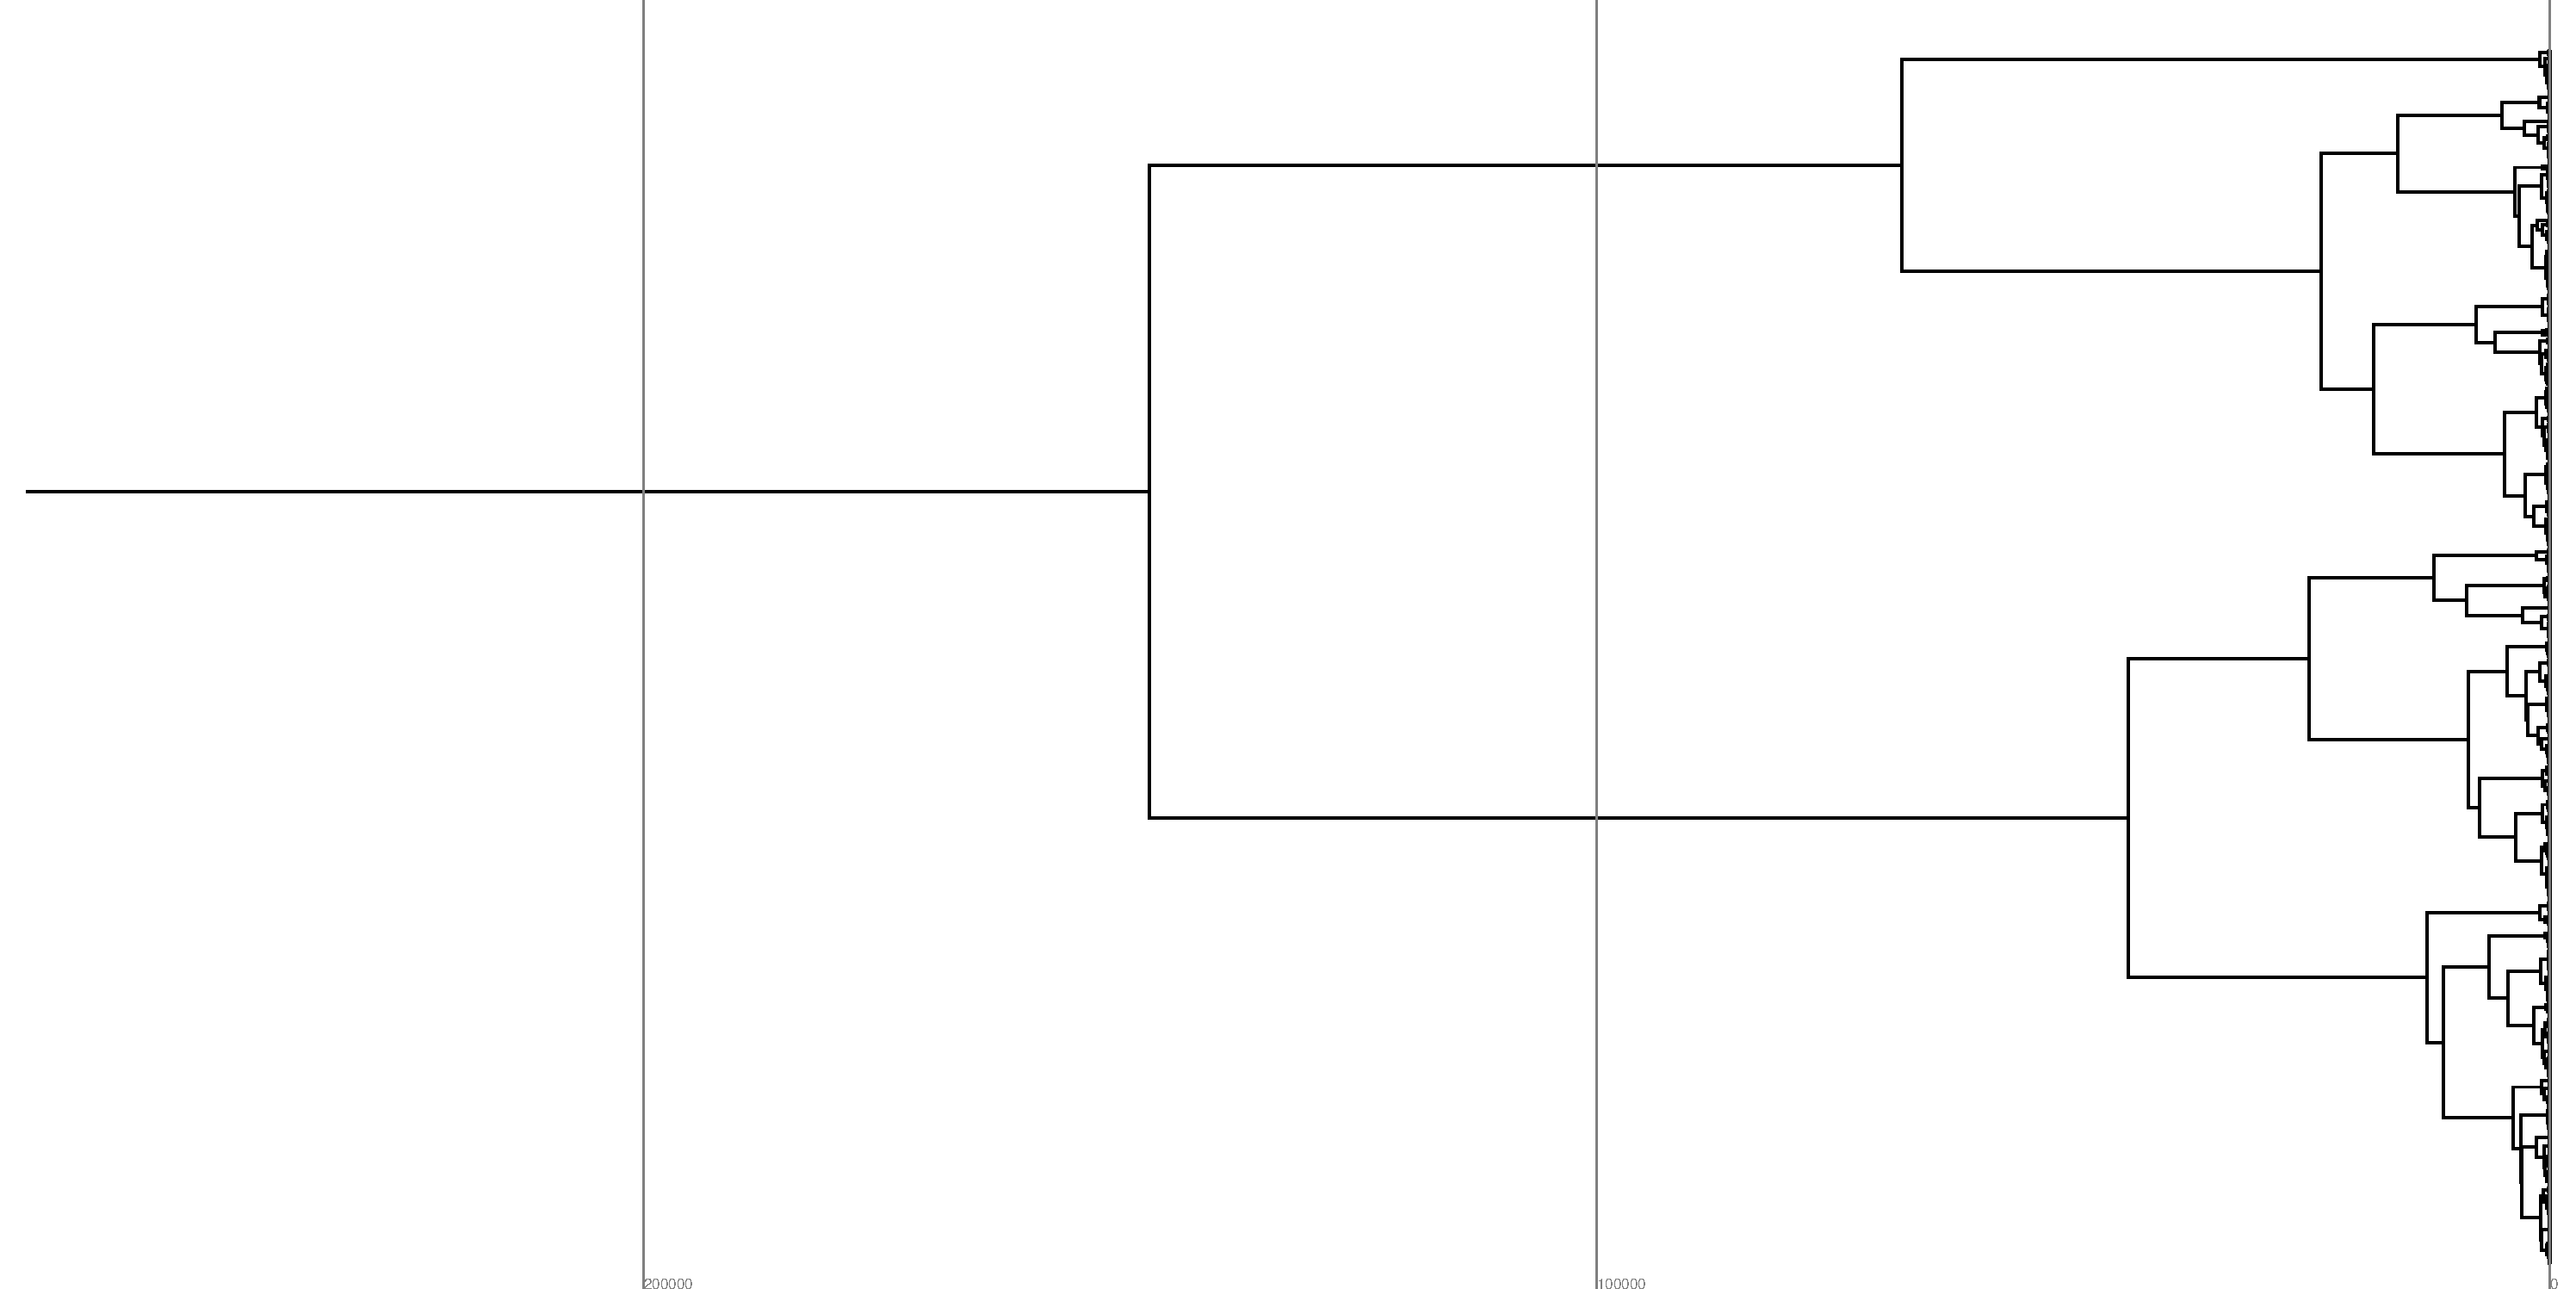
\includegraphics[height=0.12\textheight,width=\textwidth]{img/perfect-tree-phylogenies-log/epoch=7+resolution=3+treatment=4/a=collapsed-phylogeny+epoch=00007+mut_distn=np.random.standard_normal+num_generations=32768+num_islands=1+num_niches=4+p_island_migration=0.01+p_niche_invasion=3.0517578125e-08+population_size=32768+r.../eplicate=0+tournament_size=4+treatment=4+_generation=262144+_index=4+ext=.pdf}
    % \end{noindent}
    \caption{%
      4 niche ecology strong selection}
    % \label{fig:perfect-tree-phylogenies-log:TODO}
  \end{subfigure}
  \hfill
  \begin{subfigure}[b]{1\columnwidth}
    % \begin{noindent}
    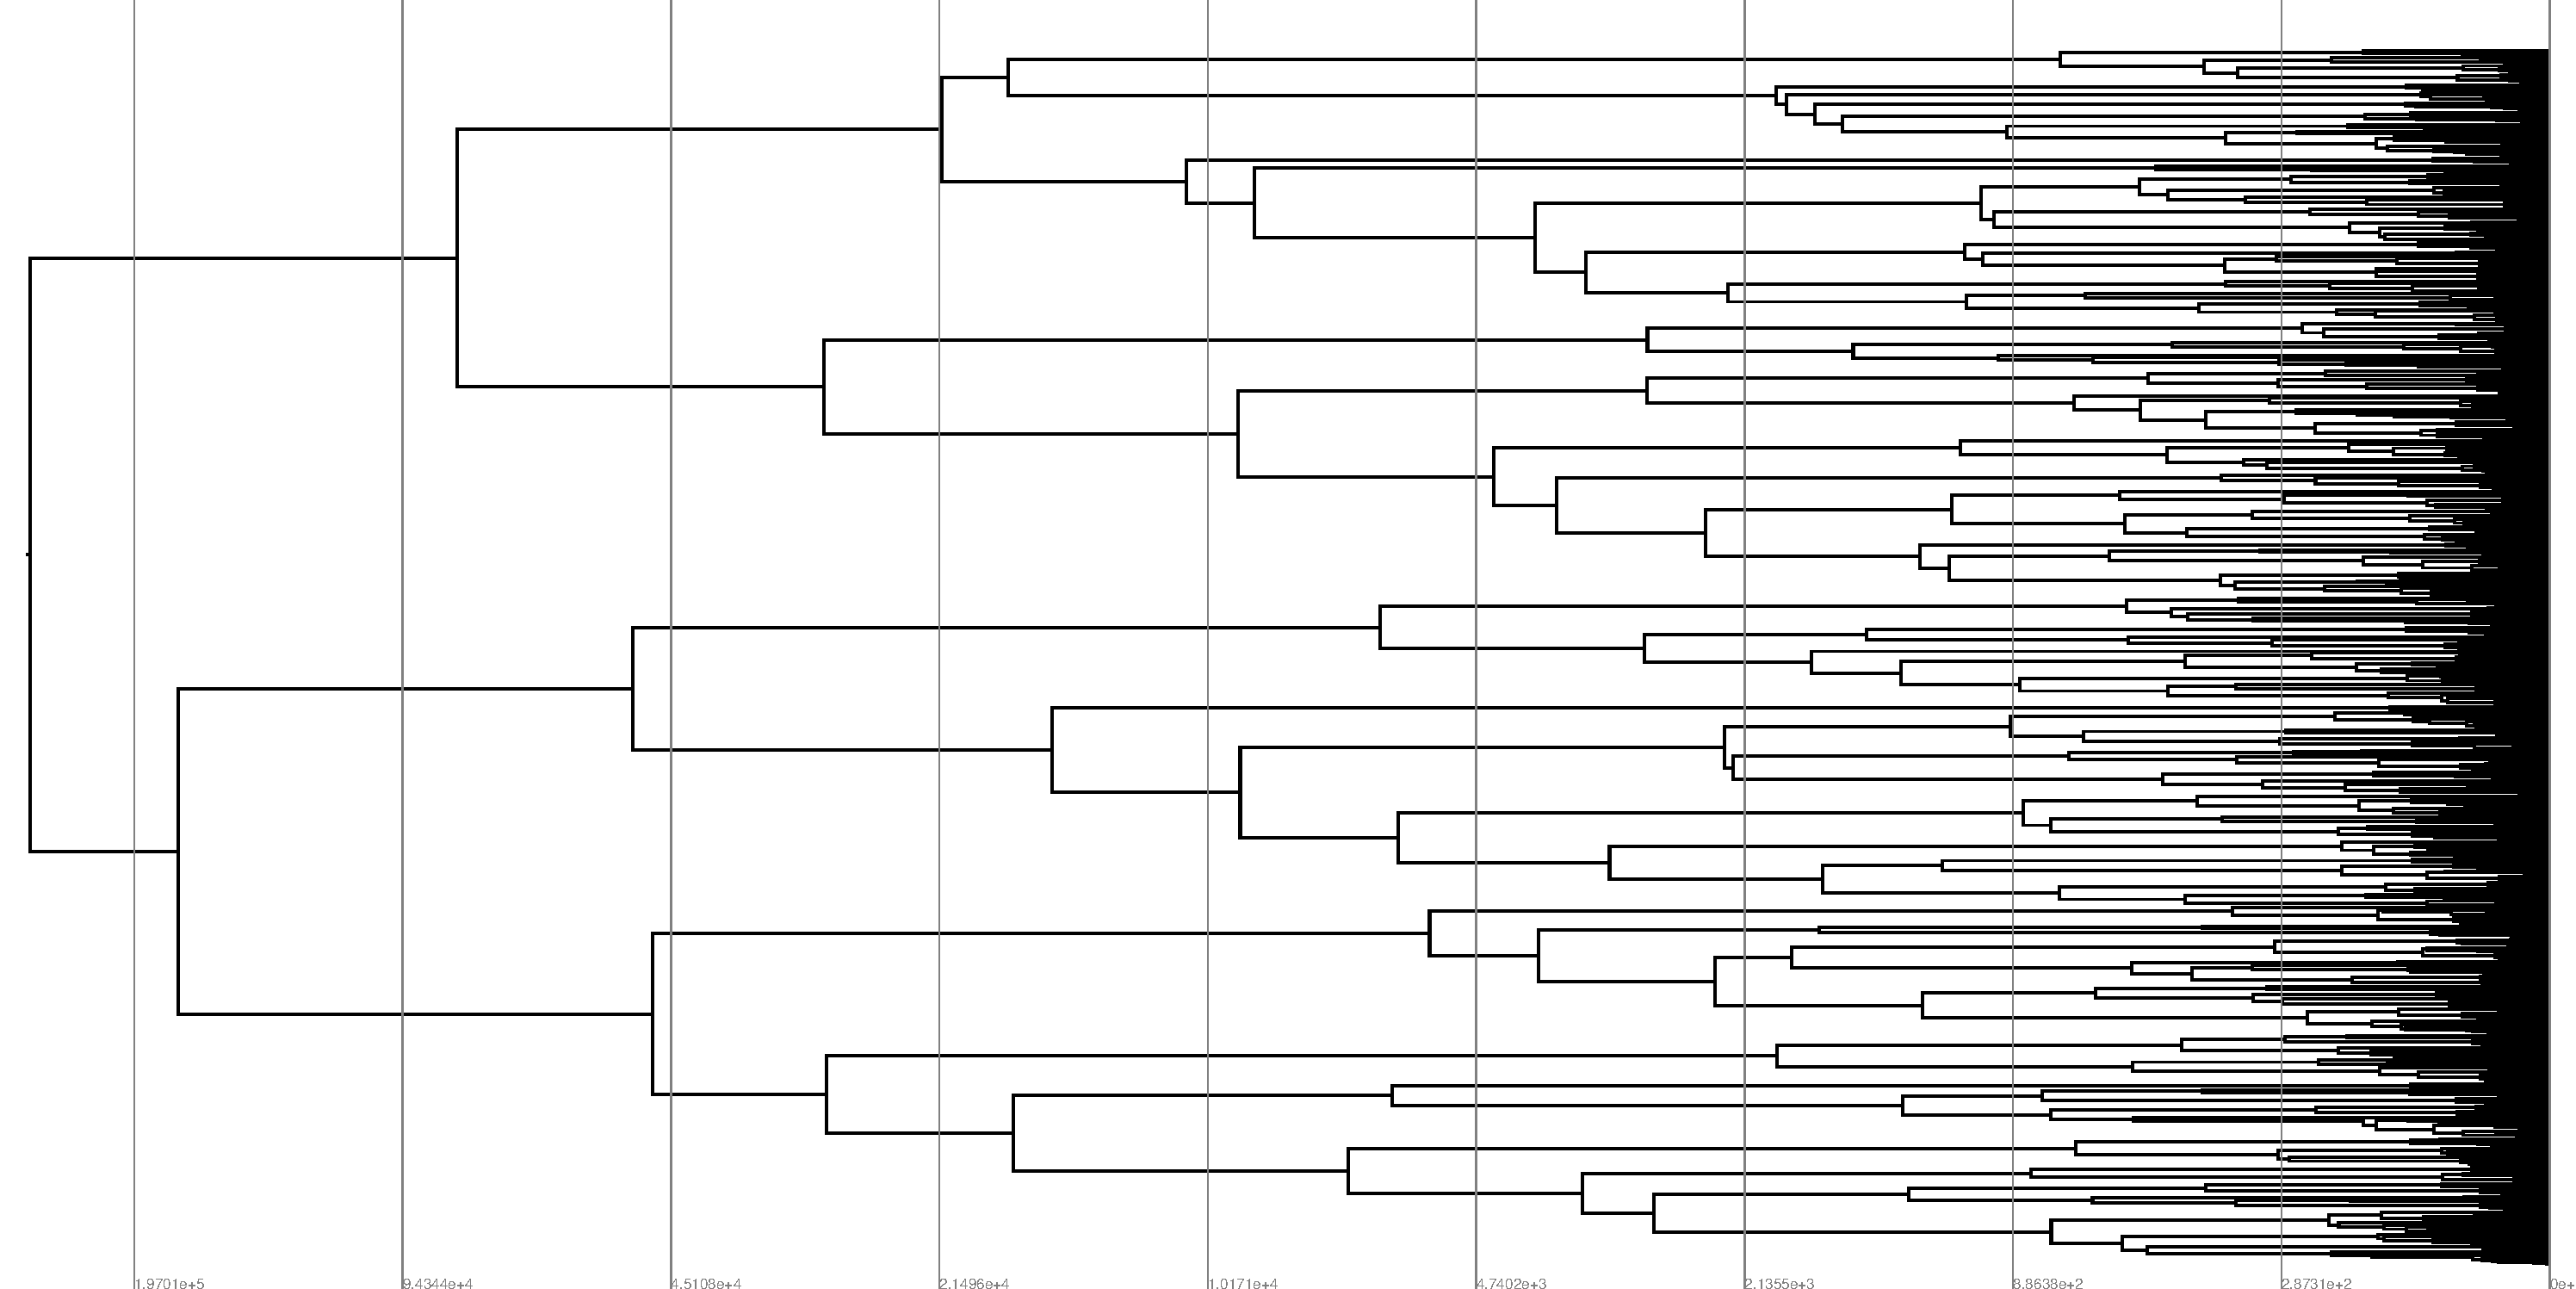
\includegraphics[height=0.12\textheight,width=\textwidth]{img/perfect-tree-phylogenies-log/epoch=7+resolution=3+treatment=6/a=collapsed-phylogeny+epoch=00007+mut_distn=np.random.standard_normal+num_generations=32768+num_islands=1024+num_niches=1+p_island_migration=0.01+p_niche_invasion=3.0517578125e-08+population_size=3276.../8+replicate=0+tournament_size=2+treatment=6+_generation=262144+_index=6+ext=.pdf}
    % \end{noindent}
    \caption{%
      spatial structure}
    % \label{fig:perfect-tree-phylogenies-log:TODO}
  \end{subfigure}
  \hfill
  \begin{subfigure}[b]{1\columnwidth}
    \centering
    % \begin{noindent}
    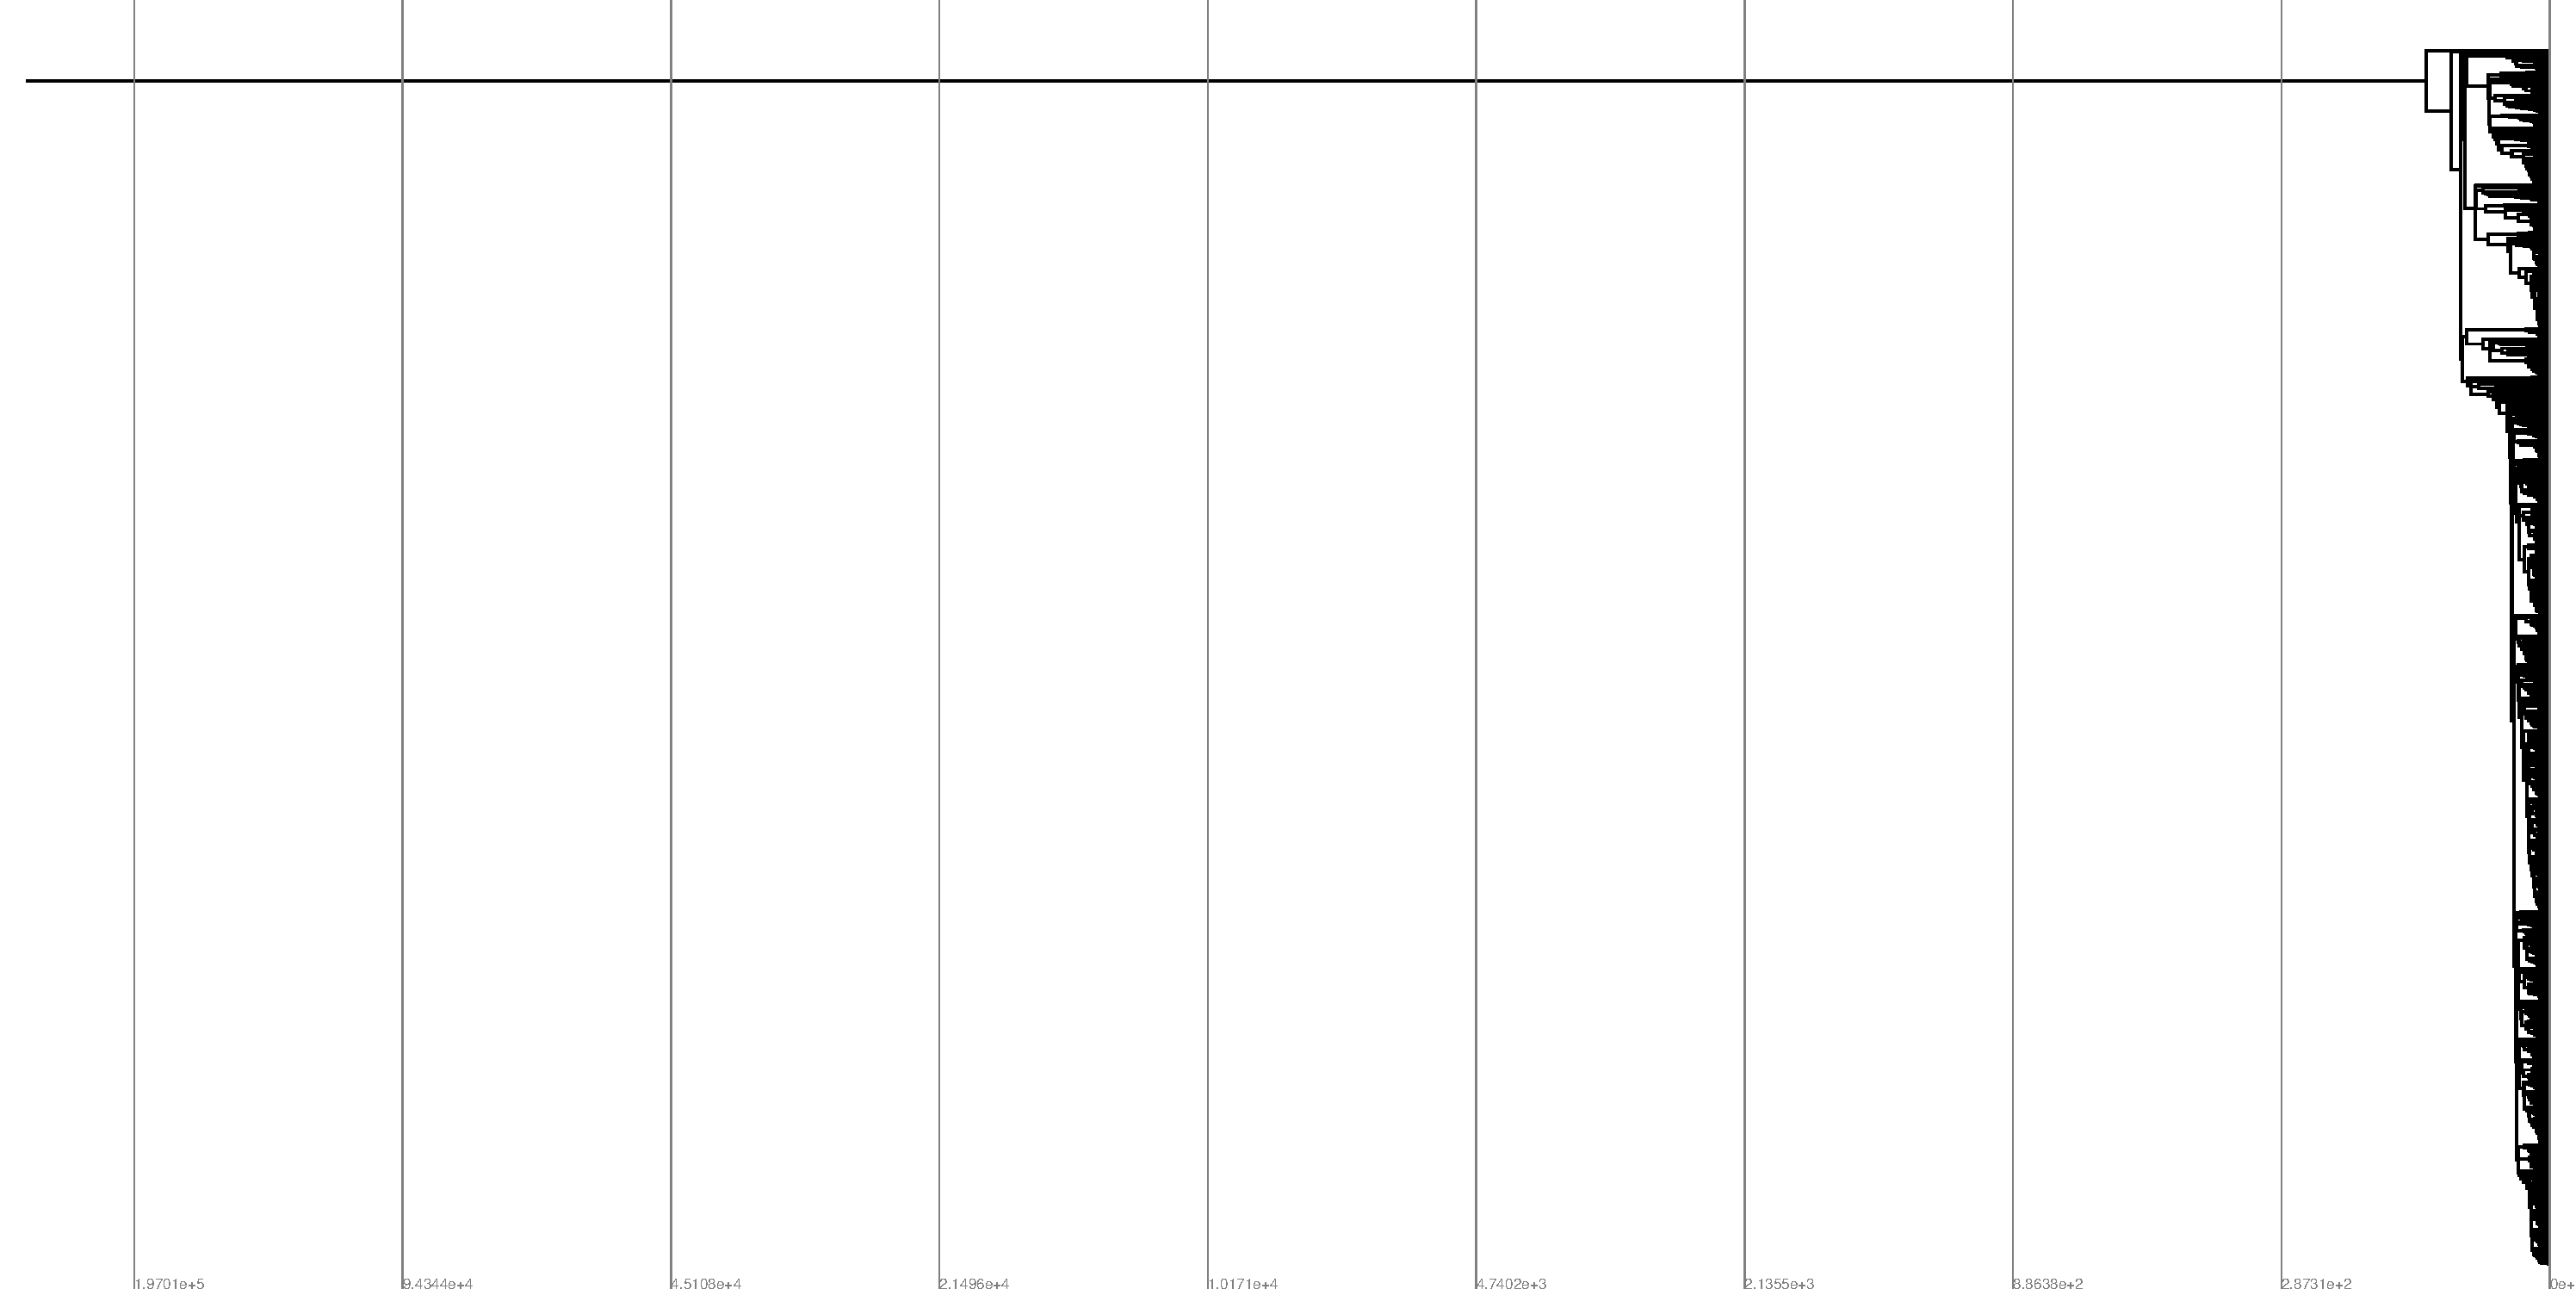
\includegraphics[height=0.12\textheight,width=\textwidth]{img/perfect-tree-phylogenies-log/epoch=7+resolution=3+treatment=8/a=collapsed-phylogeny+epoch=00007+mut_distn=np.random.standard_normal+num_generations=32768+num_islands=1+num_niches=1+p_island_migration=0.01+p_niche_invasion=3.0517578125e-08+population_size=32768+r.../eplicate=0+tournament_size=2+treatment=8+_generation=262144+_index=8+ext=.pdf}
    % \end{noindent}
    \caption{%
      plain}
    % \label{fig:perfect-tree-phylogenies-log:TODO}
  \end{subfigure}

  \caption{%
    Sample reference phylogenies across surveyed evolutionary metrics.
    Each phylogeny has 32,768 leaves.
    Note log-scale $x$ axis.
  }
  \label{fig:perfect-tree-phylogenies-log}
\end{figure*}

\begin{teaserfigure}
  \centering
  % \begin{noindent}
  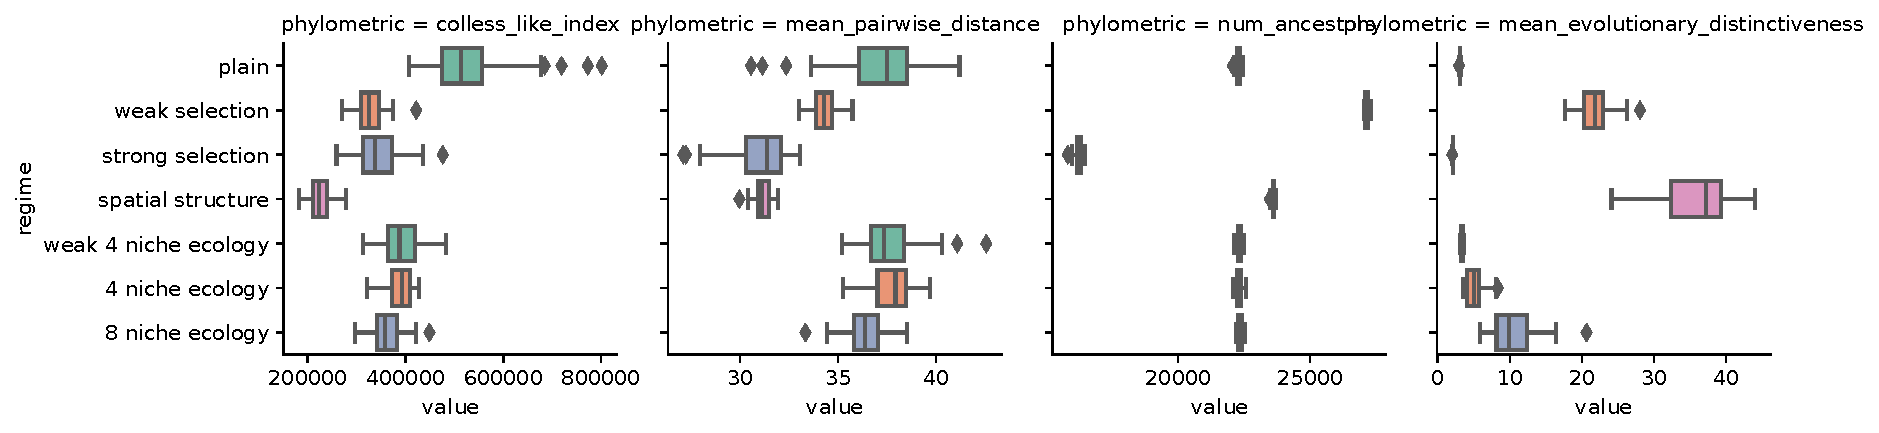
\includegraphics[width=\textwidth]{binder/binder/teeplots/col=phylometric+epoch=7+mut_distn=np.random.standard_normal+viz=boxplot+x=value+y=regime+ext=.pdf}
  % \end{noindent}
  \caption{%
    Distribution of phylometrics measured with perfect phylogenetic tracking across surveyed evolutionary regimes ($n=50$).
  }
  \label{fig:perfect-tree-phylometrics}
\end{teaserfigure}


The feasibility of harnessing phylogenetic analysis to identify evolutionary dynamics hinges on the premise that these dynamics induce detectable structure within the phylogenetic record.
Fortunately, as shown in Figure \ref{fig:perfect-tree-phylogenies-log}, dendrograms of phylogenetic histories from the different evolutionary conditions tested do indeed exhibit striking visual differences.

As a first step to characterizing the phylogenetic impact of spatial structure, ecology, and selection pressure, we tested whether surveyed evolutionary conditions exhibited detectable differences in a representative suite of four phylometrics: evolutionary distinctiveness, Colless-like index, mean pairwise distance, and sum pairwise distance.
Figure \ref{fig:perfect-tree-phylometrics} summarizes the distributions of each metric across surveyed conditions.
Statistical tests confirmed that each phylometric exhibited significant variation among surveyed evolutionary conditions for both the simple model and Avida (Kruskal-Wallis tests; all $p < 10^{-40}$; $n=50$ per condition simple model, $n=30$ Avida; Supplementary Table \ref{tab:phylostatistics-comparison-between-regimes-kwallis}).

To quantify the phylometric effects of surveyed evolutionary regimes, we performed nonparametric statistical comparisons against the ``plain'' baseline treatment.
We used a measure of distributional overlap --- Cliff's delta --- to assess effect sizes, binning into ``negligible'', ``small'' (+), ``medium'' (++), and ``large'' (+++) effects based on conventional thresholds \citep{hess2004robust}.
Significance at $\alpha = 0.05$ (*) was assessed through Mann-Whitney tests.
Figure \ref{fig:perfect-tree-phylometrics-simple-heatmap} shows nonparametric significance and effect size test results.

\textbf{Summary of Phylometric Effects}

Relative to the plain regime, all evolutionary regimes in the simple model depress the Colless-like index.
Reduction in this statistic indicates that all deviations from baseline conditions increased regularity in generated phylogenies.
This observation runs somewhat counter to prior results on similar tree balance metrics, in which the presence of spatial structure increased imbalance \citep{scottInferringTumorProliferative2020}.
One possible contributing factor is that taxa in our phylogenies were individuals, whereas Scott et al. used genotype-level abstraction (i.e., their trees were gene trees).
%Application of the metric to trees comprised individual-level taxa, instead of species-level taxa as is the case in most traditional phylogenetics work, may account for this result.
This possible effect of taxonomic unit is consistent with our results from the species-level phylogenies in the  Gen3sis system (Figure \ref{fig:perfect-tree-phylometrics-gen3sis}), in which ecological and spatial conditions elevated Colless imbalance.
Avida individual-level phylogenies were more consistent with the simple model than with Gen3sis; Colless index was significantly depressed under ecological regimes, and weakly but insignificantly depressed under spatial structure.
However, other modes of evolution did not meaningfully affect Colless-like index of Avida phylogenies.

Colless-like index is sensitive to changes in evolutionary conditions.
However, it appears to be the least useful metric in distinguishing different drivers of evolutionary dynamics, decreasing significantly under all non-plain evolutionary conditions.

Mean evolutionary distinctiveness was significantly higher under weak selection and with spatial structure than in the plain regime.
This metric significantly decreased under strong selection and under ecological regimes, but the numerical magnitudes of these effects were relatively smaller (Figure \ref{fig:perfect-tree-phylometrics-heatmap-parametric}).
We observed similar results in Avida, except no significant effect of strong selection and weak ecology was detected on the phylometric outcome.

Mean pairwise distance was significantly depressed under all regimes except ecology and weak ecology, although again the numerical magnitude of effects on ecological regimes were relatively smaller (Figure \ref{fig:perfect-tree-phylometrics-heatmap-parametric}).
Within Avida, weak but insignificant depressing effects were observed under weak selection and spatial structure regimes.
In contrast to results from the simple model, the strongest depressing effects were observed under the weak ecology and strong ecology regimes.

Finally, sum pairwise distance was significantly increased under all regimes compared to baseline, except for the strong selection regime where it was significantly depressed.
Effect size was again strongest under spatial structure and weak selection (Figure \ref{fig:perfect-tree-phylometrics-heatmap-parametric}).
Avida gave similar results, except that no significant effect was detected from the weak ecology and strong selection treatments, with a weak but insignificant increase effect detected under strong selection.

\textbf{Discussion of Phylometric Effects}

Ecological dynamics have significant influence on the surveyed phylometrics.
However, the numerical magnitudes of these effects are generally weak compared to spatial structure and selection effects (Figure \ref{fig:perfect-tree-phylometrics-heatmap-parametric}).
So, it appears careful accounting for other evolutionary dynamics (i.e., selection pressure and spatial structure) will be essential to accurate detection of ecology through phylogenetic analysis.
Mean pairwise distance may play a role in identifying ecological dynamics, as ecological dynamics --- in contrast to other factors such as spatial structure and changes in selection pressure --- have weaker effects on this phylometric.
Other phylogenetic metrics may also be better suited to detecting ecological dynamics (e.g. the ecology metric in \citep{dolson2019modes}).

Phylometric outcomes within Avida generally mirror the simple fitness model, although in many cases phylometric effects are weaker or not significant.
These less pronounced effects are not unexpected --- whereas the simple model was explicitly designed for direct manipulation of evolutionary drivers, we use more subtle configurations to impose evolutionary drivers on the Avida model (particularly, with respect to selection pressure).
Notably, the strong selection treatment resulted in no significant effects on phylometric values.
Weak selection significantly increased mean evolutionary distinctiveness and sum pairwise distance, as with the simple model, but the effect size was small.
However, spatial structure's effect size on these metrics was large and agreed with the simple model.
The ecology and rich ecology treatments agreed in sign with the simple model and generally had large effect size.
However, unlike the simple model, Avida's sole phylometric outcome under weak ecology was a strong, significant decrease in mean pairwise distance.
In contrast, the simple model exhibited no effect on this metric under the weak ecology treatment.

We additionally performed a sensitivity analysis for results from the simple model over an alternate exponential mutation operator and earlier phylogeny sampling time points.
The effects of evolutionary conditions on phylometrics were generally consistent with Figure \ref{fig:perfect-tree-phylometrics-simple-heatmap} across surveyed conditions (Supplementary Figures \labelcref{fig:perfect-tree-phylometrics-sensitivity-analysis,fig:perfect-tree-phylometrics-heatmap-sensitivity-analysis}).

\subsection{Phylometric Signatures of Ecological Dynamics in Spatially Structured Populations}

\begin{figure*}
  \centering
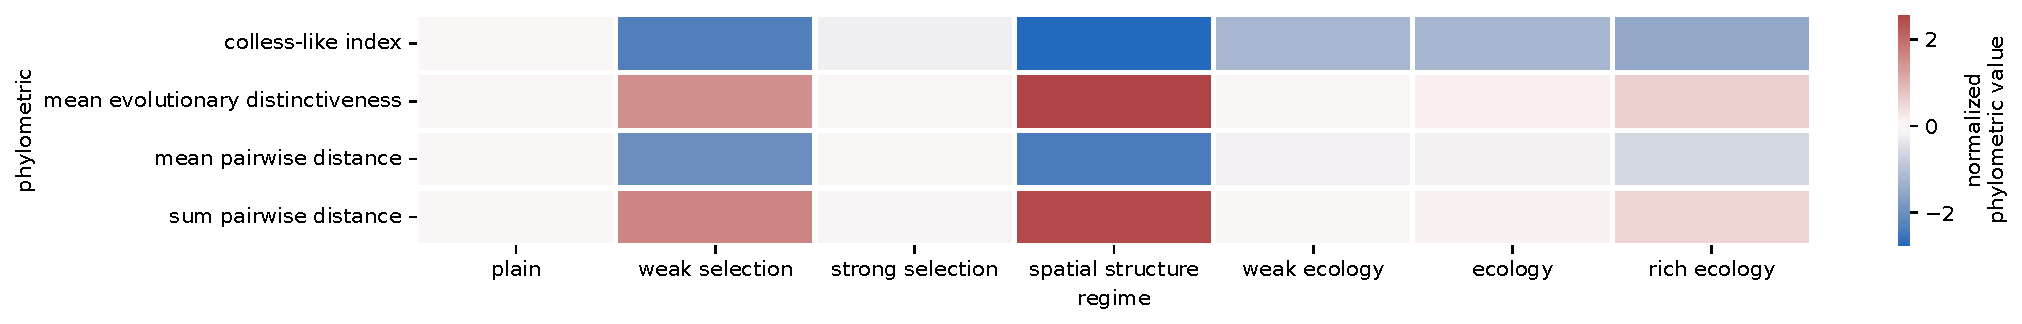
\includegraphics[width=\textwidth]{binder/binder/teeplots/epoch=7+mut_distn=np.random.standard_normal+normed=true+viz=heatmap+x=regime+y=phylometric+ext=.pdf}
\caption{%
  \textbf{Normalized phylometric responses.}
  Heatmap of normalized tree phylometrics across surveyed evolutionary regimes, calculated on perfect-fidelity phylogenies from the simple model.
  Note that normalization shows magnitude of phylometric effect beyond the point of distributional nonoverlap, unlike nonparametric normalization which tops out with complete distributional nonoverlap.
}
  \label{fig:perfect-tree-phylometrics-heatmap-parametric}
\end{figure*}


The effects of spatial structure are of particular interest, as evolution within very large populations typically entail elements of spatial structure owing to dispersal across geographic terrain.
Even within \textit{in silico} contexts, populations too large for a single processor will almost inevitably integrate spatial structure that reflects practical limitations of distributed computing hardware \citep{ackley2014indefinitely,moreno2021conduit}.
Therefore, understanding the background effects of spatial structure on the phylogenetic signatures of other evolutionary dynamics will be essential to applications of phylogenetic inference in such applications.
For this analysis, we chose to focus on ecological dynamics due to interest in how their relatively weak phylometric signatures would respond to the relatively strong influence of spatial structure (Figure \ref{fig:perfect-tree-phylometrics-heatmap-parametric}).

\textbf{Summary of Phylometric Effects with Background Spatial Structure}

\begin{figure*}
  \centering
  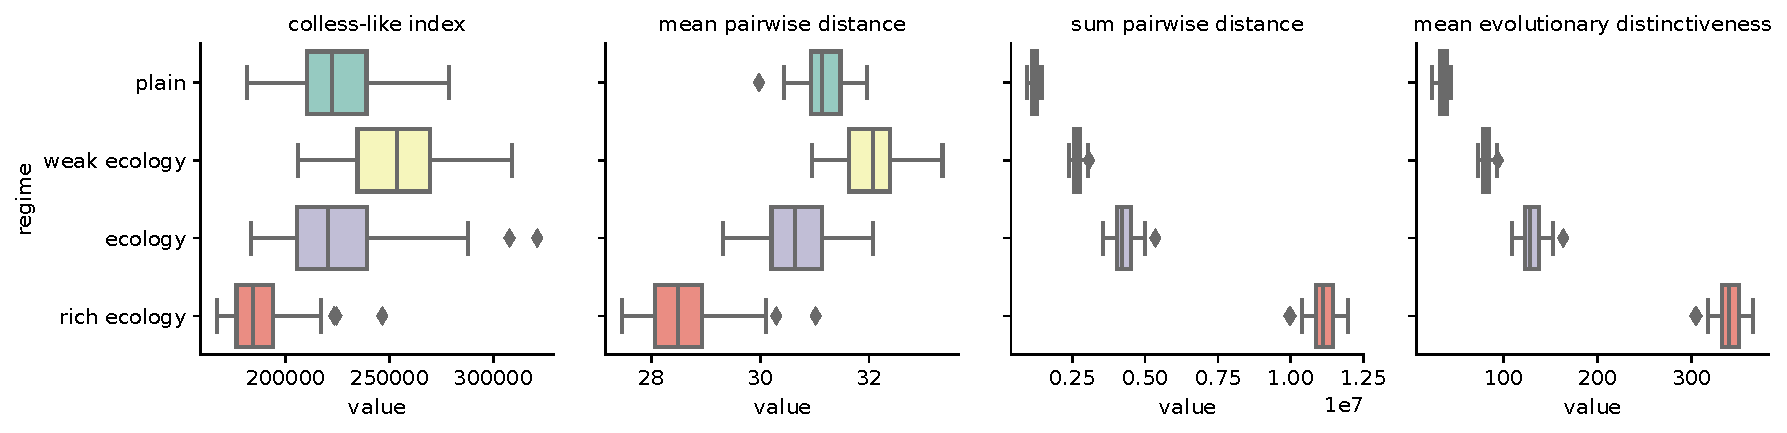
\includegraphics[width=\textwidth]{binder/binder/teeplots/col=phylometric+epoch=7+mut_distn=np.random.standard_normal+nuisance=spatial-structure+viz=boxplot+x=value+y=regime+ext=.pdf}
  \caption{TODO}
  \label{fig:perfect-tree-phylometrics-with-spatial-nuisance}
\end{figure*}


Figure \ref{fig:perfect-tree-phylometrics-with-spatial-nuisance} summarizes the distribution of surveyed phylometrics under the three surveyed ecological regimes and the control non-ecological regime, all with spatial population structure.
Statistical tests confirmed that each phylometric exhibited significant variation among these evolutionary regimes, indicating the presence of detectable structural signatures in phylogenetic structure (Kruskal-Wallis tests; all $p < 1\times10^{-8}$; $n=50$ per condition for simple model, $n=30$ Avida; Supplementary Tables \labelcref{tab:phylostatistics-comparison-between-regimes-spatial-nuisance-kwallis,tab:phylostatistics-comparison-between-regimes-spatial-nuisance-kwallis-avida}).

As in prior experiments, all ecology treatments drove significant increases in mean evolutionary distinctiveness and sum pairwise distance.
Also consistent with spatially unstructured results, rich ecology drove significant, large-effect depression of both Colless-like index and mean pairwise distance and ecology.
However, in the presence of spatial structure, the ecology treatment depressed only mean pairwise distance.
Without spatial structure, the ecology treatment depressed Colless-like index instead.
Results under weak ecology differed notably from non-spatial baseline, with all phylometrics seeing significant, large-effect increases.
Spatial-background rich ecology results from Avida agreed with the simple model.
However, significant phylometric effects were not detected from the ecology and weak ecology treatments under spatial structure conditions.

For these experiments, we again performed a sensitivity analysis over an alternate exponential mutation operator and earlier phylogeny sampling time points.
We found the effects of evolutionary conditions on phylometrics to be generally consistent across surveyed conditions (Supplementary Figure \ref{fig:perfect-tree-phylometrics-with-spatial-nuisance-sensitivity-analysis} and Supplementary Tables \labelcref{tab:phylostatistics-comparison-between-regimes-spatial-nuisance-kwallis,tab:phylostatistics-comparison-between-resolutions-allpairs-wilcox-spatial-nuisance}).

\subsection{Species-level Phylogenies from Gen3sis Model}

\begin{figure*}
  \begin{subfigure}[b]{0.5\textwidth}
    \includegraphics[width=\textwidth]{binder/binder/gen3sis/teeplots/epoch=0+mut_distn=default+viz=heatmap+x=regime+y=phylometric+ext=.pdf}
    \caption{non-spatial baseline}
    \label{fig:perfect-tree-phylometrics-heatmap-gen3sis}
  \end{subfigure}%
  \begin{subfigure}[b]{0.5\textwidth}
    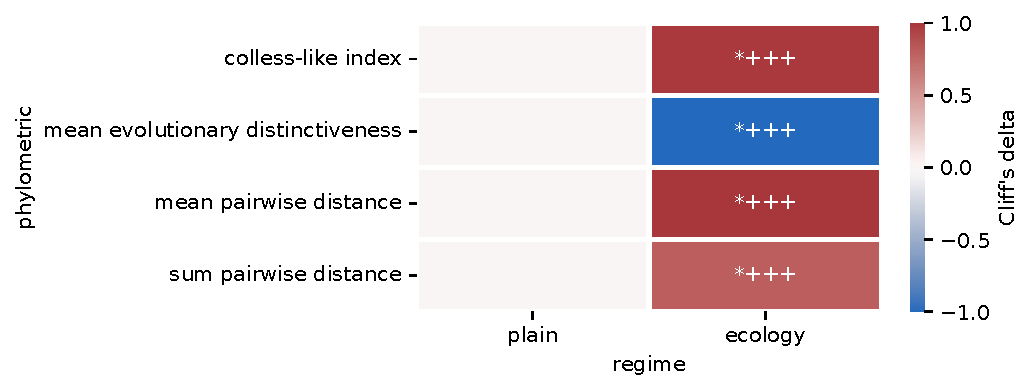
\includegraphics[width=\textwidth]{binder/binder/gen3sis/teeplots/epoch=0+mut_distn=default+spatial=true+viz=heatmap+x=regime+y=phylometric+ext=.pdf}
    \caption{spatial baseline}
    \label{fig:perfect-tree-phylometrics-spatial-heatmap-gen3sis}
  \end{subfigure}
  \caption{%
    Evolutionary regimes' effect sizes relative to ``plain'' baseline under the Gen3sis model with perfect phylogenetic tracking, normalized via Cliff's delta.
    Sample sizes $n=30$.
    Annotated +'s indicate small, medium, and large effect sizes using the Cliff's delta statistic and *'s indicate statistical significance at $\alpha = 0.05$ via Mann-Whitney U test.
  }
  \label{fig:perfect-tree-phylometrics-gen3sis}
\end{figure*}

\begin{figure*}
  \centering
\includegraphics[width=\textwidth]{binder/binder/avida/teeplots/epoch=0+mut_distn=default+viz=heatmap+x=regime+y=phylometric+ext=.pdf}
\caption{%
  Tree phylometrics across surveyed evolutionary regimes, calculated on perfect-fidelity simulation phylogenetic records.
  Note that nonparametric effect size normalization caps out to 1.0/-1.0 past the point of complete disbributional nonoverlap.
  For heatmap charts, +'s indicate small, medium, and large effect sizes using the Cliff's delta statistic and *'s indicate statistical significance at $\alpha = 0.05$ via Mann-Whitney U test.
}  
  \label{fig:perfect-tree-phylometrics-heatmap-avida-genome}
\end{figure*}

%Figure \ref{fig:perfect-tree-phylometrics-gen3sis} shows phylometric effects of spatial structure and of ecology, both with and without a spatial structure background.
Significant, large-effect changes were detected across all four phylometrics in each treatment in Gen3sis (see Figure \ref{fig:perfect-tree-phylometrics-gen3sis}).
However, with the exception of sum pariwise distance, effect signs of treatments were opposite to those for individual-level phylogenies from Avida and the simple model across all phylometrics.
Tip count effects seem likely to play a role in this discrepancy.
Unlike Avida and the simple model, which held population size constant, species richness grew freely under the Gen3sis model.
It is also possible that phylometric outcomes may be sensitive to granularity level of the taxonomic unit of the phylogeny.
As noted in Section \ref{sec:methods} and shown in Figure \ref{fig:perfect-tree-phylometrics-heatmap-avida-genome}, in Avida experiments, phylogenies using genome-level tracking (as opposed to individual-level tracking) were notably different than those using individual-level tracking.
These differences also included changes in the sign of some treatment effects, lending credence to the idea that differences between Gen3sis and the individual-level phylogenies could be partially the result of Gen3sis having a more abstract taxonomic unit.

\subsection{Phylometric Bias of Reconstruction Error}
\label{sec:phylometric-bias-reconstruction-error}

Shifting from perfect phylogenetic tracking to approximate phylogenetic reconstruction will facilitate efficiency and robust digital evolution simulations at scale, but introduces a complicating factor into phylogenetic analyses: tree reconstruction error.
A clear understanding of the impact of these errors on the computed phylometrics will be necessary for informative future phylogenetic analyses.

To explore this question, we compared phylometrics computed on reconstructed trees to corresponding true reference trees under the simple model (Wilcoxon tests; $n=50$ per condition; Supplementary Table \ref{tab:phylostatistics-comparison-between-resolutions-allpairs-wilcox}).
To err towards conservatism in detecting phylometric biases, we did not correct for multiple comparisons.
Reconstructions were performed across a range of precisions, ranging from 1\% relative resolution for MRCA estimates (most precise) to 33\% relative resolution for MRCA estimates (least precise).
Precision was manipulated by adjusting the information content of underlying hereditary stratigraphic genome annotations used to perform phylogenetic reconstruction \citep{moreno2022hereditary}.
Note that important differences exist the between nature of reconstruction error under hereditary stratigraphy versus traditional biosequence-based methods, discussed further below.

\textbf{Phylometric Sensitivites to Reconstruction Error}

\begin{figure*}
  \centering
  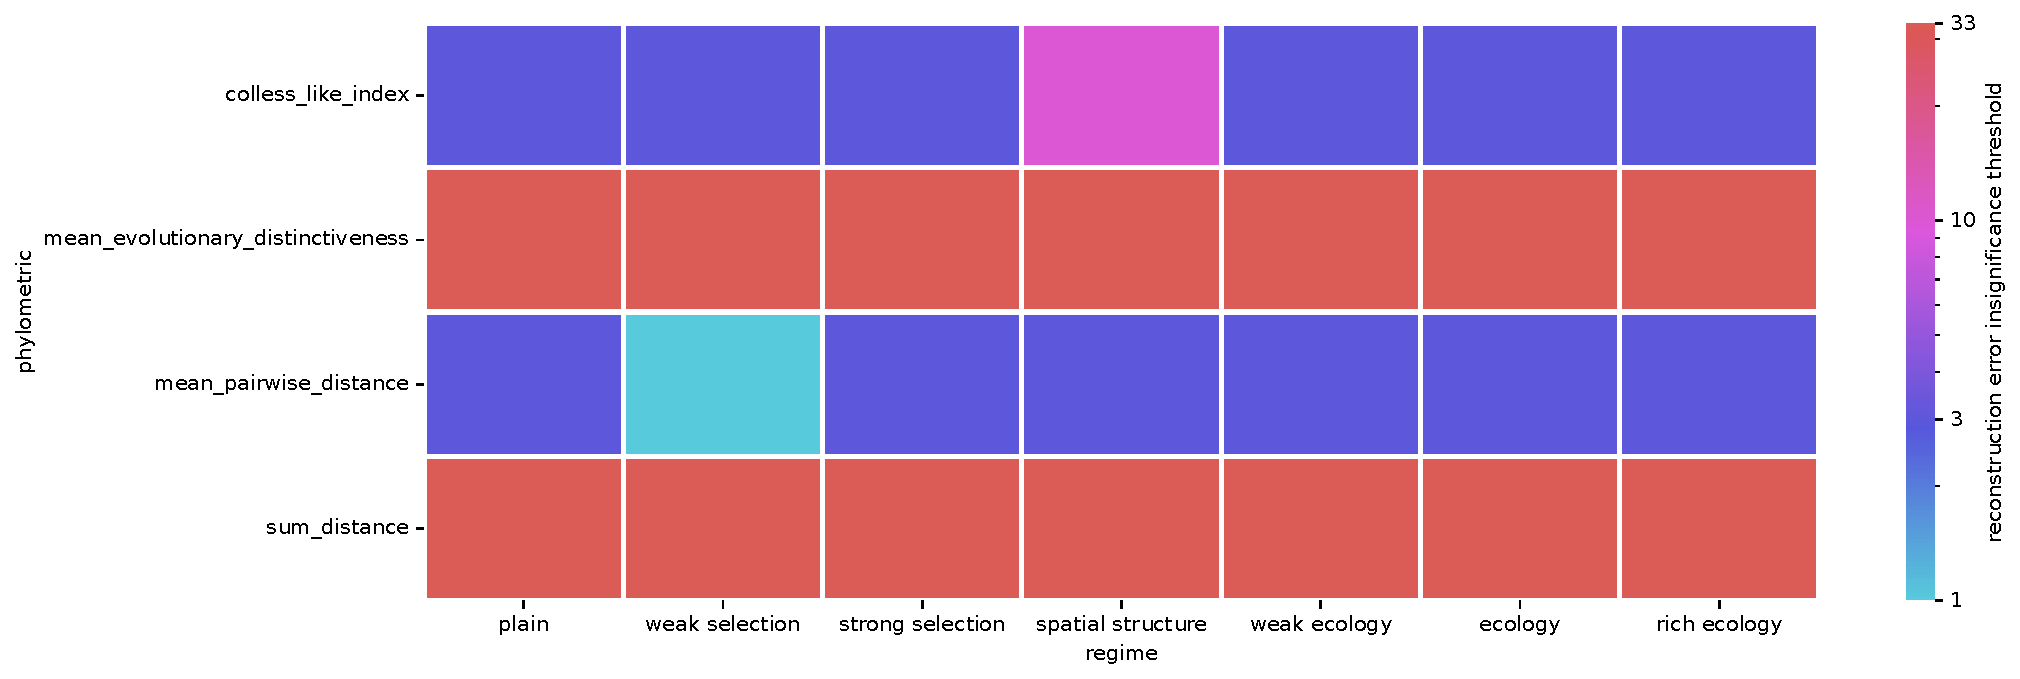
\includegraphics[width=\textwidth]{binder/binder/teeplots/epoch=7+hue=quality-threshold+mut_distn=np.random.standard_normal+viz=heatmap+x=regime+y=phylometric+ext=.pdf}
  \caption{TODO}
  \label{fig:reconstructed-tree-phylometrics-error}
\end{figure*}


For each phylometric, we sought to determine the minimum resolution required to achieve statistical non-detection (i.e., $p > 0.05$) of bias between reconstructions and their corresponding references.
For nearly all cases, 3\% reconstruction resolution was sufficient to achieve statistical indistinguishability between reference and reconstruction.
Mean evolutionary distinctiveness and sum pairwise distance were particularly robust to reconstruction error, showing no detectable bias even at only 33\% reconstruction resolution.

Phylometric sensitivity to reconstruction error was broadly consistent across evolutionary regimes.
Figure \ref{fig:reconstructed-tree-phylometrics-error} summarizes these results.

Where detectable, estimation uncertainty bias decreased all surveyed phylometrics' numerical value.
So, when testing for expected increases in phylometric values, the potential for systematic false positives due to reconstruction error can be discounted.
Supplementary Figure \ref{fig:reconstructed-tree-phylometrics} provides a full comparison of the distribution of phylometric estimates on reference trees with the distributions of phylometric estimates for reconstructed trees across reconstruction resolutions.

The relationship between reconstruction error and phylometric bias was similar under spatially structured regimes, the alternate exponential mutation operator, at earlier phylogeny sampling time points, and in the Avida model system (Supplementary Figures \labelcref{fig:reconstructed-tree-phylometrics-error-sensitivity-analysis,fig:reconstructed-tree-phylometrics-error-spatial-nuisance,fig:reconstructed-tree-phylometrics-with-spatial-nuisance,fig:reconstructed-tree-phylometrics-avida,fig:reconstructed-tree-phylometrics-error-avida}; Supplementary Table \labelcref{tab:phylostatistics-comparison-between-resolutions-allpairs-wilcox,tab:phylostatistics-comparison-between-resolutions-allpairs-wilcox-spatial-nuisance}).
Notably, however, reconstruction bias persisted at even 1\% relative resolution in some conditions of the sensitivity analysis and Avida experiments.
Forthcoming work has found that the byte-differentia hereditary stratigraphy configuration used for this experiment tends to lump closely contemporaneous lineage splitting events into a polytomy rather than a double-branching event --- i.e., indicating uncertainty rather than introducing error.
In contrast, reconstructions on single-bit differentia contain erroneously- sequenced branching rather than artifactual polytomies.
So, future work should explore whether working with single bit differentia could lessen phylometric bias.

\textbf{Detection of Evolutionary Drivers' Signatures in Reconstructed Phylogenies}

Our last objective was to assess how reconstruction error might affect detection of phylometric signatures induced by treatment conditions.
That is, we sought to perform a sort of ``integration test'' for detection of treatment conditions when working with imperfect reconstructions rather than perfect phylogenies.
To this end, we compared the phylometric outcomes of strong/weak selection, spatial structure, ecology, and weak/rich ecology relative to plain conditions for phylogenies reconstructed at 1\%, 3\%, 10\%, and 33\% resolution levels.
Supplemental Figures \labelcref{fig:reconstructed-tree-phylometrics-progressive-heatmap,fig:reconstructed-tree-phylometrics-progressive-heatmap-avida} show heatmaps with sign, effect size, and significance of phylometric effects across gradations of reconstruction precision for the simple model and Avida, respectively.
In most cases, 3\% resolution sufficed to fully recover phylometric effects of treatments observed with perfectly-tracked phylogenies.
